% -*- mode:LaTeX -*-

%% Skeleton for a thesis.
%%
%% You should not need to mess around with this file unless you want to tinker.


\documentclass[12pt]{ri_thesis}

% All packages go in here
% -*- mode:LaTex; mode:visual-line; mode:flyspell; fill-column:75-*-
% All packages used in this thesis.

\usepackage{microtype}
\usepackage{graphicx}
\usepackage{epigraph}
\usepackage[cmex10]{amsmath}
\usepackage{amsfonts}
\usepackage{appendix}
\usepackage[numbers,sort]{natbib}
\usepackage{setspace}
\usepackage{layout}
\usepackage[subfigure]{tocloft}  % Set TOC options.

% mine
\usepackage{hyperref}
\usepackage{makecell}

% For plots
\usepackage{pgfplots}
\usepackage{pgfplotstable}
\usepackage{tikz}
\pgfplotsset{compat=1.9}
\usetikzlibrary{positioning}
\usetikzlibrary{backgrounds}
\usetikzlibrary{calc}
\usepgfplotslibrary{colorbrewer}  % provided by local file.
\usepgfplotslibrary{statistics}

% Enable externalized diagrams (for final copy).
%\usetikzlibrary{external}
%\tikzexternalize[prefix=externalize-tikz/]

\usepackage[format=hang]{subfig}  % Do not include caption package in here.
\usepackage{xcolor}  % Get extra colors.
\usepackage{algorithm}
\usepackage{algpseudocode} % algorithmicx
\usepackage{ctable}
\usepackage{multirow}

\usepackage{todonotes}  % This package is slow to include.
\usepackage{xspace} % macros with trailing spaces
\usepackage{siunitx}
\usepackage[raggedright]{titlesec}  % Prevent line breaks in section titles.

% ``float'' algorithms
\usepackage{float}
\newfloat{algorithm}{tbp}{lop}

% Colors for links (except TOC -- all black).
\colorlet{documentLinkColor}{blue}
\colorlet{documentCitationColor}{black!80}
\usepackage[backref,
        pageanchor=true,
        plainpages=false,
        pdfpagelabels,
        bookmarks,
        bookmarksnumbered,
]{hyperref}
\hypersetup{
     colorlinks = true,
     citecolor = documentCitationColor,
     linkcolor = documentLinkColor,
     urlcolor = documentLinkColor,
}

% Enable capitalized references. Use this last.
\usepackage[nameinlink]{cleveref}


\input{thesis-headers}

% Page layout: approx 1" margins.
\usepackage[
  reset,
  letterpaper,
  twoside,
  vscale=.75, % Use 75% of the total vertical space (default=0.7)
  hscale=.70,  % Use 70% of the horizontal space (default=0.7)
  nomarginpar,  % No space for margin notes.
  % Margin ratio: Use default (2:3) for binding and 1:1 for on-screen.
  % hmarginratio=1:1,  % disable this for binding (more space on binding side)
  % showframe,  % enable to see the margins
  heightrounded,  % Round size of document.
]{geometry}

% Un-comment this to show a black bar by overfull hboxes.
%% \overfullrule=5pt

% Macros and color definitions.
\input{thesis-macros}
\input{thesis-colors}

\begin{document}

\frontmatter

\pagestyle{empty}

% -*- mode:LaTex; mode:visual-line; mode:flyspell; fill-column:75-*-

\title{\textbf{
Understanding forest ecology with commodity drones using semantic mapping and informative path planning
}\vspace{12pt}}
\author{David Russell}
\date{August 15, 2023}
\Year{2023}
\trnumber{CMU-RI-TR-2023-NN}

\committee{
Professor David Wettergreen, \emph{chair} \\
Professor George Kantor \\
Professor Marija Popovic, \emph{University of Bonn} \\
Kshitij Goel \\
}


\support{}
\disclaimer{}

% copyright notice generated automatically from Year and author.
% permission added if \permission{} given.
\permission{All rights reserved.}

\maketitle

\begin{dedication}
% -*- mode:LaTex; mode:visual-line; mode:flyspell; fill-column:75-*-

Athena and Marvel

\end{dedication}

\pagestyle{plain} % for toc, was empty

% The content of the thesis is broken up into many individual files.
\begin{abstract}
% -*- mode:LaTex; mode:visual-line; mode:flyspell; fill-column:75-*-

% Special indentation for abstract.
\setlength{\parskip}{1em}
\setlength{\parindent}{0em}
Drones and remote sensing can provide observations of forests at scale, but this raw data needs to be interpreted to further our scientific understanding and inform effective management decisions. This thesis studies two problems under the realistic constraint of limited domain-specific training data: tree detection for understanding carbon sequestration and vegetation mapping for forest fire mitigation.

For tree detection, we process the drone data using structure from motion and then register it to remote sensing imagery. Then, we compare different strategies for using a deep learning detector with these modalities and limited training data.
For vegetation mapping, we show that we can localize fuel that causes forest fires using image-based semantic segmentation trained on very few examples and LiDAR-based geometric reasoning. Finally, we introduce RAPTORS, a novel algorithm that plans where to collect sparse drone observations based on existing remote sensing data. We show that training a remote sensing-based vegetation classification model on observations from RAPTORS is more effective than training on observations from a coverage-based approach, especially for rare classes. 
Overall, these experiments show how using machine learning, data harmonization across scales, and intelligent sampling can facilitate automated forest understanding with limited training data.
%These approaches could inform data-driven forest management, which is critical in this time of rapid environmental change.

%We explore how to best detect trees using co-registered data from remote sensing, drone surveys, and manual observations of tree locations. We use a pre-trained deep learning model to detect trees in drone and aerial data and propose a multi-scale fine tuning process to increase performance. 
%We first fine-tune the model for the drone data, using the sparse but accurate field reference measurements, then use the predictions on the entire region surveyed by the drone to fine-tune a model for remote sensing data that has broad coverage.
%To map vegetation structure and type, we combine image-based semantic segmentation models and geometric reasoning from SLAM to build metric-semantic maps of the environment. 
%Finally, we introduce RAPTORS, a novel informative path algorithm that that is suitable for low-cost consumer drones because it can plan the entire mission before takeoff.
%RAPTORS leverages existing remote sensing data using unsupervised feature extraction, determines uncertain regions with Gaussian Process modeling, and plans a path using a sampling-based approach.

%We find that tree detections on remote sensing data are improved by the multi-stage fine-tuning process compared to the base model or single-stage training .
%We show that the mapping system can generate a map that accurately classifies vegetation type using a surprisingly-few number of training images.
%We evaluate RAPTORS by planning drone flights to collect observations of land cover, to train a classification model using remote sensing data. We demonstrate that a model trained on observations from RAPTORS generates better predictions of rare classes than a model trained on observations from a baseline coverage planner. A commonality of these experiments is that a small quantity of highly-relevant data can be critical for automating forest understanding. Additionally, combining observations from different modalities can yield more accurate and scalable predictions, which is critical in this time of increasing environmental change.





%Forests are undergoing rapid changes driven climate change, land use changes, and invasive species. Humans are often tasked with management decisions, with goals such as preserving biodiversity, improving carbon sequestration, or reducing the risk of wildfire. Unfortunately, land managers rarely have high quality quantitative data to inform these decisions. Examples include the location or species of tree or a map of the predominant vegitation type.
%Field work is labor intensive and only allows a small subset of a region to be surveyed. Satellite data can provide effectively-unlimited coverage, but suffers from low spatial resolution which impedes the quality of automated prediction systems. Unmanned aerial systems or "drones" represent an effective middle ground between this two currently-used approaches. Drones can cover a larger area than a forester can with minimal human effort and provide orders-of-magnitudes higher resolution than satellite data. Furthermore, drones can be deployed on demand, to provide timely information about a recent event such as a fire, as opposed to satellite data which can take weeks or months to re-observe a region. 

%The robotics community has sought to apply drones to forestry in a variety of settings. However, this work focuses on highly-engineered multi-sensor drones that perform extensive online processing. This technology is simply not ready for deployment by land managers, who frequently lack dedicated technical staff. However, the commercial drone market has made great strides in usability over the last decade and drone surveys are pervasive in many domains such as agriculture, surveying, and inspection. Due to the robust commercial and open source ecosystem, forestry is seeing an increasing adoption of automated drone surveys. These are often executed autonomously using a coverage plan which is configured before the mission. Then, data is fed into a photogrametery software which produces colored 3D meshes or pointclouds of the scene, using geometric computer vision. 

%This thesis aims to make two contributions. The first is a flexible full-mission planner which prioritizes observing a diverse set of observations. This is especially useful in situations where there is imbalanced distribution of classes or a classes are clumped spatially. The second is supplementing the existing geometric mapping with semantic information. This could be something like the type or species of the vegetation.

\noindent
\end{abstract}

\begin{acknowledgments}
% -*- mode:LaTex; mode:visual-line; mode:flyspell; fill-column:75-*-

% Special indentation for acknowledgments.
\setlength{\parskip}{1em}
\setlength{\parindent}{0em}

\noindent
I am sincerely grateful to Prof. George Kantor, Prof. Marija Popovic, and Kshitij Goel for taking the time to serve on my committee for their time and insightful feedback. And especially to my advisor, Prof. David Wettergreen, for all the suggestions, direction, encouragement and understanding. I appreciate both your willingness to let me explore and ability to direct my focus to what matters.

To my labmates, Srini Vijayarangan, Rohan Zeng, Ananya Rao, Maggie Hansen, and Abby Brietfield. Thank you for all the discussions about research and real life. You taught me a lot and made this far more fun.

Much of this work happened in close collaboration with the SafeForest team: Dr. Francisco Yandun, Winnie Kuang, and Duda Andrada. I appreciate the numerous times you have provided me useful data, helped me debug code, or clarify my thoughts. 

%To Eric Schneider, anything I've discussed with you has given . Your organization and preparedness will never cease to amaze me.  

To Dr. Derek Young and Dr. Mike Koontz at Open Forest Observatory, I appreciate your perspectives on how this work really gets done. 

To the directors of the Robotics Institute Summer Scholars program, Prof. John Dolan and Rachel Burcin. Thank you for going above and beyond to make opportunities for me and so many others. I would not have been here without you.

\end{acknowledgments}

\begin{funding}
% -*- mode:LaTex; mode:visual-line; mode:flyspell; fill-column:75-*-

% Special indentation for funding acknowledgments.
\setlength{\parskip}{1em}
\setlength{\parindent}{0em}
Safeforest \\
AIIRA \\
NSF SBIR? \\

\end{funding}

% Table of contents: Make links black, add a hyperlink target, and disable
% microtype (as per the docs).
\cleardoublepage

% Set the space before & after header line for the Contents, List of tables,
% List of figures. This is primarily to make the Contents will fit on two pages.
\setlength{\cftbeforetoctitleskip}{3.0em}
\setlength{\cftaftertoctitleskip}{2.0em}
\setlength{\cftbeforeloftitleskip}{3.0em}  % LOF: List of figures
%\setlength{\cftafterloftitleskip}{2.0em}  % For some reason leave this out.
\setlength{\cftbeforelottitleskip}{3.0em}  % LOT: List of tables
%\setlength{\cftafterlottitleskip}{2.0em}  % Same
\cftsetpnumwidth{1.75em}  % Prevent overfull hbox on TOC numbers.

\hypersetup{linkcolor=black}  % Make TOC links black.
\hypertarget{contents}{}
\microtypesetup{protrusion=false}
\tableofcontents
\chapternote{\hspace{-12pt}When this dissertation is viewed as a PDF, the page header is a link to this Table of Contents.}
\clearpage
\listoffigures
\clearpage
\listoftables
\microtypesetup{protrusion=true}


% Main matter. Use
\mainmatter
\pagestyle{thesis}

\hypersetup{linkcolor=documentLinkColor}  % Make links colorful again

% ********************************************************************************
%                                  Main Content
% ********************************************************************************

% Main content: 1.5 line spacing.
\onehalfspace
% -*- mode:LaTex; mode:visual-line; mode:flyspell; fill-column:75-*-

%% Include all contents; each chapter should be a separate file.

% -*- mode:LaTex; mode:visual-line; mode:flyspell; fill-column:75-*-

\chapter{Introduction} \label{chapIntroduction}
Forests impact many aspects of our life on earth, ranging from the altering composition of the atmosphere, purifying water, moderating local temperature, and contributing to fire risk. Unfortunately, they are under threat from a variety of factors including climate change, invasive species, fire, and direct human pressures \cite{IPCC2019ClimateReport}. This is causing forests to change at an unprecedented rate. In light of these rapid changes, it is critical that we have up-to-date information to inform decisions such as habitat preservation, sustainable timber operations, forest fire mitigation, and carbon sequestration. In this work we specifically study aspects of forest fire mitigation and carbon sequestration, though the approaches aim to be generic enough to scale to other applications. 

There are many sources of data that can be used to inform forest management. In this work we study three: manual field measurements, data from drones, and remote sensing imagery. The manual measurements are accurate and granular, but fail to provide information at scale. Conversely, remote sensing data can provide information at scale, but lacks fine-grained spatial detail and is challenging to interpret. Drone data strikes a middle ground between these extremes. The goal of this work is to develop techniques that leverage all three sources of data to produce insights about forests that are both accurate and scalable.
\section{Research Questions}
Our broad goal of multi-modality forest understanding motivates three specific areas of study:
\begin{itemize}
    \item How can data from field surveys, drones, and remote sensing be integrated to accurately detect trees at scale?
\end{itemize}
\begin{itemize}
    \item How can drones be used to classify vegetation type in a large forested region?
\end{itemize}
\begin{itemize}
    \item How can sparse drone surveys be planned to provide the most diverse and informative measurements about a region?
\end{itemize}

%\section{Methods}
%\section{Conclusions}
%Most traditional cameras only capture three different bands of light, red, green and blue. In contrast, many space-borne sensors capture more spectral bands and are termed either multi- or hyper-spectral. Multispectral data has coarse bands with gaps between them, while hyperspectral data has many small bands which observe a near-continuous spectral signal \cite{Lu2019ComparingProperties}. These sensors vary widely in spatial resolution with legacy government satellites such as Landsat 8 and Sentinel 2 having resolutions of multiple meters per pixel. More recent commercial offerings have pushed the resolution to the sub-meter range. 


%In this work, we focus on optical data, since it is conceptually most similar to what we capture from drones. This data is collected by an electro-optical sensor which takes images of the earth. Then, the images are registered together and referenced into absolute geospatial coordinates. This process relies on the estimated pose of the platform when the image was taken, the height of the ground, and manual corrections. From there, an orthographic render is generated. This is a projection of the data into a top-down view, which is commonly aligned with the axes of geospatial coordinate system used to define the location. Many satellite data sources capture bands outside of the visible wavelength. Sensors which capture a x to y number of bands are termed multi-spectral and sensors which captured y to z bands are termed hyper-spectral. 
%\begin{itemize}
%    \item talk about what what sat is 
%    \item Sat data has a broad extent and may be too low res
%    \item Reannalysis has shown that accuracy is often very low \cite{} 
%    \item Data products from crewed aircraft has higher resolution but require substaintial investment and planning
%\end{itemize}

%Another option is "grid coverage" where a lawnmower pattern is executed twice, in perpendicular directions. An important consideration when executing these surveys is the drone altitude, which represents a trade-off between coverage ability and spatial resolution. While drones can in theory fly to a substantial altitude, they are restricted in the US to 400ft and below due to concerns about interfering with crewed aircraft. The final consideration is front- and side-overlap. Front overlap refers to the fraction of the image which is observed in two consecutive frames captured as the drone is flying forward. The side overlap refers to how much overlap there is between neighboring flight lines.


% -*- mode:LaTex; mode:visual-line; mode:flyspell; fill-column:75-*-

\chapter{Background \& Related Work} \label{chapBackground}
\section{Motivation}
Forests impact many aspects of our life on earth, ranging from the composition of the atmosphere, purification of water, moderating local temperature, and contributing to fire risk \cite{IPCC2019ClimateReport}. Unfortunately, they are under threat from a variety of factors including climate change, invasive species, fire, and direct human pressures. This is causing forests to change at an unprecedented rate. In light of these rapid changes, it is critical that we have up-to-date information to inform decisions such as habitat preservation, sustainable timber operations, forest fire mitigation, and carbon sequestration. In this work we specifically study aspects of forest fire mitation and carbon sequestration, though the approaches aim to be generic enough to scale to other applications. 

\subsection{Forest Fire Mitigation} 
Destructive forest fires have increased dramatically over the past decades \cite{spreading_like_wildfire, ayanz2021, nfn2022}. This is due in large part to climate change, which leads to hotter and drier weather along with stronger winds \cite{spreading_like_wildfire}. This has also led to increased forest mortality from pests expanding their range, such as the mountain pine beetle in the Western US \cite{Jenkins2014AndFuels}. Humans have also contributed more directly to fires by suppressing small fires which causes fuel to build up over time. Finally, there is an increase in ignition sources from careless human activity and infrastructure such as power lines. These fires are now more dangerous to humans and property because of their scale and speed as well as increasing habitation in close proximity to forests, termed the urban-woodland interface. The ecological consequences of fire are also increasingly dire. Historical fires were a natural part of the ecosystem and the vegetation was able to regenerate due to surviving trees and un-burned seeds. The intensity of modern fires completely destroys all vegetation, making it much harder to for regions to regrow. This can lead to erosion and eventual transition from forest to grassland.

It is becoming increasingly clear that reactive firefighting is insufficient to combat fires of this magnitude and preemptive mitigation efforts are required. One way to actively reduce the risk of destructive fires is by fuel management, or removing dense understory vegetation \cite{Fire2021FuelsManagement, WildlandFireResiliencyProgram20214Plan, Agriculture2019HazardousComplex}. This is a challenging problem due to the sheer area of forested land and the limited resources currently put toward preemptive efforts \cite{spreading_like_wildfire}.
There has been increasing government interest in technological innovation, with the USDA \cite{USDA2023USDAGrant} and NASA \cite{SPSO2023Research2023} releasing grant funding opportunities. These specifically address the need for pre-fire understanding and mitigation efforts. 
Since feul management is physically demanding and requires specilized knowledge, there are increasing concerns about labor shortages \cite{CommisionGlobalDivision}. This has led proposed robotic systems that can supplement human efforts by semi-autonomously removing vegetation \cite{couceiro2019semfire}. In many of these applications, a key step is understanding the current location of fuel in the environment. This can be useful for prioritizing which regions to target, especially when using an automated system that may have limited situational awareness. Furthermore, it can inform fire-fighting strategies if the region succumbs to fire. Therefore, one of our main objectives is to map what type of vegitation is where in the environment.

\subsection{Forest Carbon Sequestration Prediction}
The other problem we explore in this work relates to assessing carbon sequestration in forests. This is relevant because forest biomass is a key carbon sink \cite{Griscom2017NaturalSolutions}. Understanding this sequestration is important for our general understanding of likely climate futures, and also to aid in the fight against climate change. Carbon offsets or "credits" have emerged as a contentious tool in the fight against climate change and the eventual goal of net-zero emissions. They allow an entity (an individual, corporation, or government) to pay a carbon credit vendor to offset their emissions by sequestering or stopping the generation of a comparable amount of emissions. This is motivated by the unfortunate reality that change cannot happen imediatly and some activities are much more challenging to de-carbonize than others. It is expected that demand for carbon credits will rise by a factor of 50 by 2050 according to a McKinsey report \cite{Blaufelder2021AChallenge}. 

Unfortunately there is widespread skepticism that this process truly offset the released carbon due to a variety of factors. The first is "carbon leakage" or the fact that carbon may be temporarily sequestered but released over time. This is especially relavebt for nature-based carbon capture solutions, such as when a forest burns due to wildfire. The second is "additiveity", which states that a carbon credit may be issued even though a behavior wasn't changed. For example, a credit could be issued for preserving the carbon in a forest, even though the carbon would not have been released even if the credit were not issued. The final issue is simple miss-estimation in the ammount of carbon sequestered. Unfortunately, it has been shown that this error is a systematic overestimate of the true carbon stock \cite{Badgley2022SystematicProgram,West2020OverstatedAmazon}. While technology cannot address all the issues with carbon accounting, it can make validation more scalable and objective. In this work, we take a first step toward automated carbon estimation by accurately detecting individual trees in satellite imagery. This can allow us to apply tree-level modeling based on predicted attributes such as species and height to estimate biomass.    


\section{Current Approaches for Informing Forest Management}
\subsection{Manual Forestry Measurements}
Understanding forests is still a largely manual process where foresters go into the field and measure various quantities such as tree height, diameter, density, species. In commercial contexts this is often called timber cruises \cite{ServiceFSHHANDBOOK} and in ecology it is often called forest inventories \cite{USForestServiceDepartmentofAgriculture2016FORESTPLOTS}. This process is a extremely laborious and means that only a limited area can be surveyed.


\subsection{Remote Sensing}
Remote sensing data is captured by sensors onboard satellites or airplanes and is rapidly becoming a critical tool for environmental monitoring \cite{Parra2022RemoteMonitoring}. This is because of the large spatial regions that are observed by these sensors which can span up to global converge in the case of some satellites. This data can take many forms ranging from light detection and ranging (LiDAR) \cite{LiDARForestryBeland2019}, synthetic aperture radar (SAR) \cite{Hall2020WhatEarthdata}, and electro-optical (EO) data. Electro-optical data is obtained from electro-optical is the class of sensors that include traditional cameras. Most traditional cameras only capture three different bands of light, red, green and blue. In contrast, many space-borne sensors capture more spectral bands and are termed either multi- or hyper-spectral. Multispectral data has coarse bands with gaps between them, while hyperspectral data has many small bands which observe a near-continuous spectral signal \cite{Lu2019ComparingProperties}. These sensors vary widely in spatial resolution with legacy government satellites such as Landsat 8 and Sentinel 2 having resolutions of multiple meters per pixel. More recent commercial offerings have pushed the resolution to the sub-meter range. 


%In this work, we focus on optical data, since it is conceptually most similar to what we capture from drones. This data is collected by an electro-optical sensor which takes images of the earth. Then, the images are registered together and referenced into absolute geospatial coordinates. This process relies on the estimated pose of the platform when the image was taken, the height of the ground, and manual corrections. From there, an orthographic render is generated. This is a projection of the data into a top-down view, which is commonly aligned with the axes of geospatial coordinate system used to define the location. Many satellite data sources capture bands outside of the visible wavelength. Sensors which capture a x to y number of bands are termed multi-spectral and sensors which captured y to z bands are termed hyper-spectral. 
%\begin{itemize}
%    \item talk about what what sat is 
%    \item Sat data has a broad extent and may be too low res
%    \item Reannalysis has shown that accuracy is often very low \cite{} 
%    \item Data products from crewed aircraft has higher resolution but require substaintial investment and planning
%\end{itemize}

\subsection{Drone Surveys}
Unmanned aerial vehicles or drones were initially developed by the millitary. Over the last decade, a variety of companies have begun to offer drones for a variety of domestic applications. This was driven by decreased costs and minuterization of the drone platforms as well as high-performance, low SWaP cameras which have quickly become the most common sensors on small drones. Drones have become increasingly prevalent in agriculture and forestry because of their low cost, ease-of-use, high spatial resolution, and on-demand coverage. 

\section{Automated methods for understanding forest structure}
\subsection{Offline: Photogrametry}
In general, commodity drones produce only monocular images with potentially a low-accuracy GPS and orientation estimate. A common approach for estimating geometric from this type of data is photogrametry, also known as structure from motion or 3D reconstruction. The origins of photogrametry date back to WWII where it was a manual processed to estimate the geometry of structures from aerial images. Modern automated approaches began todo. Preliminary reconstructions of realistic large-scale scenes began with academic work such as \cite{Agarwal2009}. Over the last decade, numerous commercial and open-source software have been developed to accomplish the task. Some examples include: Agisoft Metashape, COLMAP, OpenMVG, OpenDroneMap.

The details vary by application and assumption, but a common pipline is the following. First, distinctive features are detected in each image. These represent small patches of pixels which are likely to be distinctive, such as corners and edges. Then, features are matched between images, based on the local appearance. 
Given these correspondences, multiple things can be estimated. The first is the location of these matched points in the 3D space, using triangulation between the cameras. The second is the location of the cameras. Finally, if the camera isn't accurately calibrated, it's common to estimate the parameters which describe how points in the world appear on the image. Given the interplay between all of these elements, it's critical to estimated them together in a global joint optimization. The class of techniques for solving this problem are termed bundle adjustment and are often build on iterative nonlinear least squares. 

After these quantities are estimated, it's common to re-estimate the correspondences between images using the existing solution as a way to filter incorrect correspondes which are not consisent with the majority of other matches. These steps are often the focus of extensive engineering effort to improve the final performance. 

After this iterative process converges, the result is a sparse output consisting of the camera locations and calibration parameters as well as a sparse set of 3D locations. This sparse representation doesn't capture the full geometry of the scene, since only the most distinctive points are represented. Moreover, because it is a pointcloud, we cannot reason about which parts of the scene would obstuct or "occlude" the view of another one. To accomplish these tasks, we leverage the fact that many solvers can produce a mesh representation of the surface of the scene. A mesh is a common representation in computer vision and graphics, which consists of a set of 3D points connected by triangular faces. 

The process of mesh computation varies by solver. A common first step is to estimate the likely depth to the surface from each camera using color constancy. This means that for a set of posible distances, the observed color from that camera is checked against the color which would be observed by the other camera, if that were the true location of the surface. From this information, a predicted most likely depth surface is predicted for each pixel. Then, the predicted depth is combined across all cameras to produce a consistent 3D geometry. This is often done using a truncated signed distance function representation \cite{} 

\begin{figure}
    \centering
    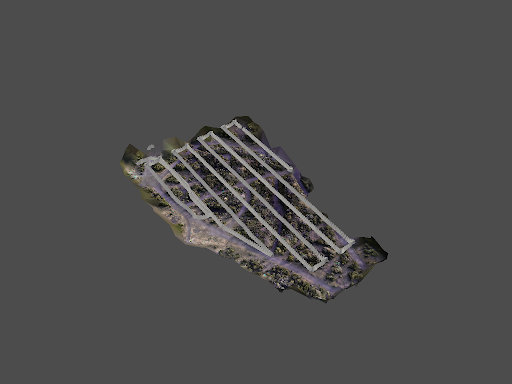
\includegraphics[width=\textwidth]{figs/methods/structure_from_motion/camera estimation.png}
    \caption{The estimated camera locations in space}
    \label{fig:camera-locations}
\end{figure}

These solvers are becoming increasingly robust, and are well-suited to reconstructing scenes captured by drone surveys because the same location is often seen across many images.

\subsection{Online: Simultaneous localization and mapping}
Structure from motion is a powerful tool, but a key limitation is that it can only be used to map the environment after a mission is complete. In settings where a drone is operating autonomously in complex environment such as under the canopy, it is important that it understands where it is in relation to obstacles in real time. This problem is challenging because it requires completing two challenging tasks at once: building a map of the world while estimating where the robot is within the map. This problem is known in the robotics literature as simultaneous localization and mapping (SLAM). This refers to the fact that in a new environment, the robot must build a map of the world at the same time as figuring out where it is in this map. 


Talk about SLOAM \cite{Chen2020SLOAM:Inventory}, a semantic mapping approach specifically for forestry 

%\begin{itemize}
%    \item Should we include more about survey-based methods?
%    
%\end{itemize}


\section{Automated methods for understanding attributes of forests}
Given the increasing amount of raw data about our forests, a key question is how to extract meaningful insights. Quantities such as the extent, species composition, health, or biomass of a forest can be more easily used to make management decisions. Automated processing methods can free domain experts from the laborious task of interpreting this data by hand. There has been a steady shift from methods which are hand-designed to those which use supervised machine learning. This means fitting some sort of model to existing data that shows the input information and the correct interpretation. Then this model can be used to generate predictions on new data. Over the last decade there have been an explosion of approaches relying on deep learning \cite{Lecun2015DeepLearning}, which is a subset of machine learning using models that have multiple hiararchical processing steps. This requires dramatically more parameters than previous machine learning models but allows greater flexability and expressivity. This means that less human intuition is required but also means that large quantities of labeled data are expected to achieve good performance. 



\subsection{Determining Types and Location of Vegitation}
The end goal of an automated forestry system is often to produce a map of where different classes are. Since the predictions are initially made on each image, an important step is inferring the 3D location of these predictions from the 2D image and also resolving disagreeing predictions for the same location. This challenge has been addressed by many approaches in both geospatial and robotics reserach. A key distinction between approaches in these fields is often whether incremental maps need to be produced as the system is running. In geospatial applicaitons, it's often assumed that the data can be processed in a batch after the mission is completed. In robotics context, the content in the environment often informs the exploration, so the maps must be built in realtime. 

Davila et. al. uses a high-precision GPS-INS to register images \cite{Davila2022ADAPT:AI}


\subsection{Understanding What is in Images}
Semantic segmentation is the task of assigning a classification label to every pixel in an image. In the forestry domain, these classes could be broad, such as trees, shrubs, and grasses or more granular, such as different species of trees. An example image can be seen in Figure \ref{fig:background:semantic_seg_example}.

\begin{figure}
    \centering
    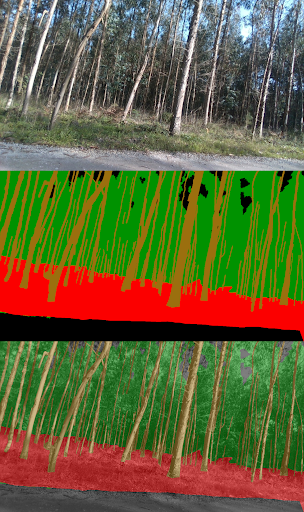
\includegraphics[width=0.45\textwidth, trim={0 340px 0 0}, clip]{figs/background/automated_understanding/segmentation_example.png}
    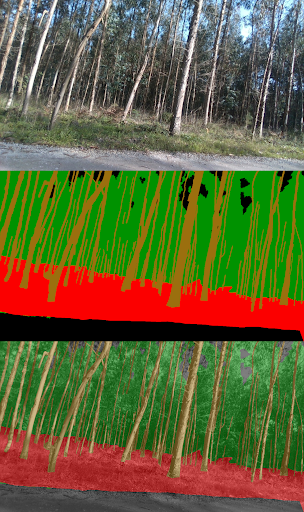
\includegraphics[width=0.45\textwidth, trim={0 170 0 170}, clip]{figs/background/automated_understanding/segmentation_example.png}
    \caption{A visualization of the goal of semantic segmentation. The input image is on the left, and the desired output is on the right, color-coded by class. Red is understory fuel, green is canopy, brown is trunk, and black is background such as bare earth and sky}
    \label{fig:background:semantic_seg_example}
\end{figure}

An early work on semenatic segmetation with deep learning was Fully Convolutional Network \cite{Shelhamer2017FullySegmentation} which took early insights from image classificaiton and adapted them to give per-pixel class predictions. Shortly following this was U-Net \cite{RonnebergerUNET2015}, which had an encoder-decoder architecture with skip connections to preserve high-resolution details. A wide variety of approaches have been developed since then using slight variations on these initial concepts. A recent shift has been toward using transformers \cite{Vaswani2017AttentionNeed} which has resulted in work such as Segformer \cite{Xie2021} and SegNext \cite{Guo2022SegNeXt:Segmentation}.

A signifcation fraction of semantic segmentation works were evaluated on datasets related to autonmous vehicles, sch as CityScapes \cite{Cordts2016}. However, these methods have been shown to be applicable to other domains, and recent work has explored them in the context of drone forestry images \cite{Nogueira2017SemanticConvNets, Neves2020SemanticU}. 


There are a variety of different approaches to semantic mapping that assume different sensors, goals, and domains \cite{Kostavelis2015SemanticSurvey}.
A common toolbox for generic semantic mapping Kimera \cite{Rosinol2020} that provides many different approaches.

To the best of our knowledge, one of the first works that explores semantic mapping in a forestry context is \cite{Andrada2022IntegrationRoboticsb}. This work also studies identifying forest fire fuel   

\begin{itemize}
    \item Talk about what we mean by semantic mapping 
    \item Talk about some generic approaches: UFO map \cite{Duberg2020UFOMap:Unknown}, Kimera 
    \item Our semantic mapping \cite{RussellUnmannedMitigation} that was derived from \cite{semantic_slam_RGBD}
    \item Talk about land-use mapping approaches from ecologists \cite{Liu2018DeepClassification} 
\end{itemize}


\subsection{Detecting Trees from Over-Canopy Data}
A key first step in many ecological modeling applications is understanding the location and extent of individual trees. Because of this, the problem of detecting trees in drone and satellite has recieved signifcant attention. There are a variety of approaches and one way to classify them is whether they use geometric or visual information about the scene. 

Talk about CHM approaches

We chose to use DeepForest \cite{Weinstein2020DeepForest:Delineation} in this work because it's a commonly-used approach that was trained on a diverse set of trees from the national ecological observation network (NEON) \cite{Keller2008ANetwork} across the country.

Talk about DetectTree2 \cite{DetectTree2} \\
Go through Derek's paper and find other ones.

\section{Planning informative drone surveys}

In many forestry applications, the region of interest is commonly substantially larger than what is feasible to survey, either by hand or even with a drone. In practice, foresters  select a small set of plots to visit and extrapolate from these sparse observations to the entire region. These plots are chosen using expert knowledge of the region to be diverse and representative.

Despite the ability of drones to cover much large regions than humans alone, they still fall short of the ability to perform  exhaustive coverage. For example, rough calculations suggest that it would take a drone pilot 250 full days flying to survey the TODO region. Therefore, it is clear that judicious use of limited resources is critical.

Satellite or aerial data is the primary modality of data that scales to the extent required for understanding forests at scale. Unfortunately, prior work has shown that many existing satellite prediction models are highly inaccurate \cite{}. Furthermore, useful global models exist only for select satellite data product and for common tasks like biomass estimation. Therefore, they are not applicable when improved satellites are launched or if a regional satellite or aerial campaign is conducted.
It is possible to tackle fine-grained tasks such as species classification with satellite data, but they are often only relevant to a small region \cite{Sweden}. 
Therefore, we wish to streamline the process of developing satellite prediction models by using a generic framework and fitting it to local observations.

Specifically, we assume that our drone collects data that can be accurately interpreted to predict the quantity of interest. For example, we can task a human annotator with identifying tree species from high-resolution drone images, or train a deep learning model to do the same. We further assume that information relavent to this task is contained in remote sensing data of the scene, but it's not easy or scalable to label this data directly. This may be because a human labeller does not possess the intuition to label species based solely on low-resolution satellite data. This claim is especially relevant if the remote sensing data contains channels other than Red-Green-Blue, as it is hard for humans to fully interpret this data \cite{Hard to label multispectral}.

Given these assumptions, the goal is to choose a set of sample locations to observe with the drone. From these observations, we obtain a classification label for each observed pixel in the remote sensing data. We then train a satellite prediction system using these observed pixels as the ground truth training examples. The goal of this work is to observe regions which serve as useful training samples for this satellite prediction system. This is similar to the ideas of active learning \cite{Ren2022ALearning}, where a repository of unlabeled data is available and an algorithm can query an oracle for labels of a subset of samples. However, active learning is not directly applicable to our domain since in classical formulations, any combination of samples can be selected. In this work, the samples relate to spatial regions that must be visited by a drone. Therefore, it must be possible to visit all the requested samples subject to operational constraints such as the drone's battery life.

This problem is most closely related to prior work in informative path planning (IPP). This diverse field is concerned with how and were to sample observations with an agent to gain some understanding of a phenomena of interest. Due to the diversity of application domains which have their own specific objectives, assumptions, and constraints, there are a diversity of approaches tackling this broad problem. For our domain, a desirable informative path planning algorithm:

\begin{itemize}
    \item \textbf{Considers non-spatial features:} Since we assume that we have prior satellite or low-resolution aerial data of a scene, it is important that an intelligent algorithm leverages this information.
    \item \textbf{Plans over a long horizon:} The commodity drones considered in this work must execute a plan developed prior to launch, e.g. offline, and cannot replan in-flight.
    Therefore, it is important that the algorithm can produce a plan which can be executed for many observations sequentially, ideally as many as can be taken before the battery must be replaced. 
    \item \textbf{Is computationally fast and scalable:} We desire that this algorithm can be executed on a laptop in the field to enable easy deployment.
    To be operationally useful, it must be possible to develop a plan for a new---potentially large---region in a short period of time.
    \item \textbf{Considers area measurements:} Many informative path planning algorithms assume that an observation is a single point in space. Instead, we want to plan were to observe with a downward-facing camera or where to survey a small region. In either case, these observations cover a region that is too large to be approximated as a single point.
\end{itemize}



\subsection{Online methods}

Significant work has been done under the assumption that the agent can re-plan its trajectory online, based on the observations it sees during execution. This requires a sophisticated robotic platform that can sense its environment, process this data into a useful format, re-plan which regions would be useful to explore, and execute this plan. In most cases, the agent maintains some sort of belief of which regions uncertain, desirable, or combination of both. At each re-planning iteration, the agent seeks to develop a plan that is likely to optimize its objectives within the operational constraints such as path length.

The work of \cite{Popovic2020} proposes a generic framework for terrain monitoring with UAVs equipped with a downward facing camera. This work assumes that the quantity of interest is a scalar field defined over the environment that has spatial correlations, e.g. similar locations will have similar values. The example use-case is modeling the density of weeds in an agricultural application, where it is most important to accurately model regions with a high infestation. Further, it assumes that the UAV is able to re-plan its trajectory in flight, after taking uncertain measurements of the environment. A strength of this work is that it models the altitude-dependent effects of a drone camera: at higher altitudes the camera can observe more area but the quality of the measurements will be lower. Using an optimization-based framework and a probabilistic sensor model, the algorithm plans a sequence of observations that decrease the uncertainty while focusing on regions of high predicted weed density. This first part of this path is followed until a new plan based on new observations is developed. This approach is shown to be more effective than a uniform coverage plan at a fixed altitude because it can predict which regions will have more weeds and spend more of the sensing budget there. An extension of this work \cite{Stache2021AdaptiveSegmentation} further explores these concepts with real data. Specifically, they use semantic segmentation to identify weeds in the images and fit empirical models to the segmentation accuracy at different altitudes. This work also shows higher accuracy than a non-adaptive baseline. In both cases, a fundamental strength of the approach is the reason we cannot use it in our domain---online re-planning based on the observed data is critical to the performance increase over the baseline.

A key feature of the previous work is that it seeks to model only regions that were observed with the drone. The main decision is how many times to re-observe a region and at what altitude. In our setting, we wish to make observations with a drone and extrapolate beyond them with satellite data. This goal is somewhat related to that of \cite{Ruckin2022}, which seeks to plan a drone flight that collects images to train a deep learning model for land use classification. In this setting, it is assumed that the drone has a downward facing camera that observes a scene. It also possesses a deep learning model that predicts the land use for each pixel, as well as a measure of uncertainty about the prediction. The goal is to collect images, that when labeled by a human annotator after the mission, can be used to update the model the deep learning model so its performance is better on new data. The authors show that collecting images that the current model is uncertain about leads to better performance after retraining. Therefore, when the drone is collecting data, it should prioritize images that the current model is uncertain about. As the drone explores a region, it generates the uncertainty predictions for each observed images, but cannot access the true label. Then, it continuously updates plan that tries to observe new uncertain images, by assuming that unobserved images next to uncertain observed images will also be uncertain. As with the prior work, this approach requires online reasoning to be effective. Furthermore, this approach has a subtly different goal from ours: their goal is to collect images that can be used to train a good model for new drone observations whereas our approach assumes a model exists already for drone data and these predictions can be used to inform a satellite model. 

Some prior work formulates the problem in similar way to our objective. Work by Kodule et. al. \cite{Kodgule2019Non-myopicMeasurements} and an extension by Candela et. al. \cite{Candela2020PlanetaryMapping} explore the problem of where to gather information with a planetary robot, e.g. Mars Rover, given that the whole region has already been observed by a low-fidelity orbiting satellite. Specifically, it is assumed that the world is represented as a grid of pixels each containing a multispectral (8-channel) observation. Then, multiple Gaussian Processes \cite{Rasmussen2004} are defined which uses the spectral values at each pixel as well as the spatial location of each pixel as features. The goal of 

%Due to the assumption of prior imagery, we may leverage approaches from \cite{Candela2021}, which uses an MCTS planner to explore a world for which prior satellite data exists. This work uses a Gaussian Process to model a quantity of interest. It is challenging to directly apply this work because it assumes that each pixel can be regressed individually by the Gaussian Process. This assumption is unlikely to be correct for high spatial and low spectral resolution data since texture within a local neighborhood will likely need to be considered.

%that can be used to gather information to train a good model for satellite data
%Alberto's Planetary , Alberto's Coral \cite{Candela2021}
%Yogi's Coral \cite{Jamieson2020ActiveEnvironments},


\subsection{Offline/batch methods}
\begin{itemize}
    \item \textbf{Ergodic} Ananya's sparse sensing \cite{Rao}
    \item \textbf{Generic} Sankalp's \cite{Arora2017RandomizedConstraints}, Daniela Rus' Correlated orienteering \cite{Yu2016CorrelatedTasks}
    \item \textbf{TIGRIS} \cite{Moon2022TIGRIS:Planning}
    In this work the authors use a sampling based approach. The chance of taking a sample is biased toward those locations which have higher information content. Importantly, this work takes into account the s
\end{itemize}

Ergodic planning, specifically sparse-sensing ergodic planning \cite{Rao}, provides a framework to plan samples over an \textit{information map} which describes how likely each sample is to be valuable. We could derive this information map from the current model prediction in multiple ways. For example, we could specify that samples predicted as rare classes or extreme AGB values are more interesting. Or we could estimate model uncertainty using ensembles or monte-carlo dropout. However, this approach only considers a per-sample interestingness and spatial diversity of samples. In this case, diversity of appearance may matter more than diversity of location. 



\begin{table}[]
\resizebox{\columnwidth}{!}{%
\begin{tabular}{|l|l|l|l|l|l|}
\hline
 & \makecell{Sparse \\ Ergodic \\ Sensing \cite{Rabbi2020Small-ObjectNetwork}} & \makecell{Optimization-\\based \\ replanning \cite{Popovic2017OnlineUAVs}} & TIGRIS \cite{Moon2022TIGRIS:Planning} & \makecell{MCTS on \\ GPs \cite{Candela2020PlanetaryMapping}} & Proposed \\ \hline
\makecell{Non-spatial \\ features} & X & X & X & Y & Y \\ \hline
\makecell{Long horizon} & Y & X & Y & Y & Y \\ \hline
\makecell{Fast \& scalable} & Y & Y & Y & X & Y \\ \hline
\makecell{Area \\ measurements} & X & Y & Y & Y & Y \\ \hline
%\makecell{Incorporates \\ non-trivial \\ dynamics} & Y & Y & Y & N & N \\ \hline
\end{tabular}%
}
\caption{A comparison of the capabilities of existing informative path planning algorithms.}
\label{tab:my-table}
\end{table}

We can apply concepts from online approaches to offline approaches
We can close the gap between online and offline approaches 



\chapter{Methods} \label{chapMethod}
\section{Datasets}
In this work we use data from a variety of sources. The first is from small, consumer-grade drones that capture only GPS-tagged images. This is relatively easy to collect and representative of what is commonly available in forestry. The second type of data is from a custom drone payload that records data from multiple sensors at once. To the best of our knowledge, this is one of the first instances of collecting data with all of these sensors. The third type of data is existing data from remote sensing, specifically an aerial mapping survey. This data is freely available. Finally, we use annotated forestry data that was captured below-canopy. We uses this as training data for our system.

\subsection{Commodity Drone Data}


In this work, we use several sources of commodity-level drone data. The first is actually collected with our more sophisticated drone. In these experiments, we only use the images from one camera and geo-tag them with our payload GPS. This is a reasonable analog for commodity drone data, since our camera and GPS are comparable to what would be found on a small commodity platform. 

The second set of data we use in this work collected with a Mavic Air 2s, a small commodity drone. The drone was flown in a lawnmower pattern at 100 meters in Vermont. Data was taken in two separate locations. 
%The second source of data is taken from a study of structurally-complex western conifer forests \cite{Young2023}. This data was collected with a DJI Mavic in a lawnmower pattern at an altitude of 120 meters.

\subsection{Multi-Sensors Drone Data}
Many modern approaches to simultaneous localization (SLAM) and semantic mapping require as input multiple sensing modalities, such as cameras, LiDAR, IMU, and GPS. Therefore, other members of our team built a modular, multi-sensor payload that could be mounted on a drone. A render of the payload can be seen in Figure \ref{fig:methods:payload}. 

\begin{figure}
    \centering
    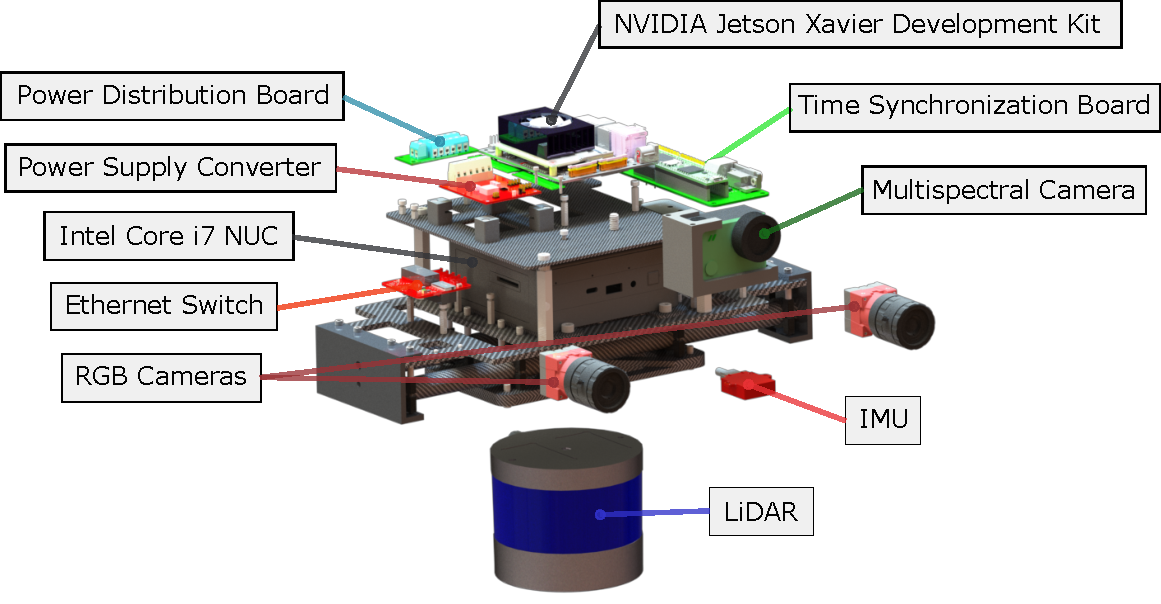
\includegraphics[width=0.55\textwidth]{figs/methods/datasets/payload_annotated.pdf}
    \hfill
    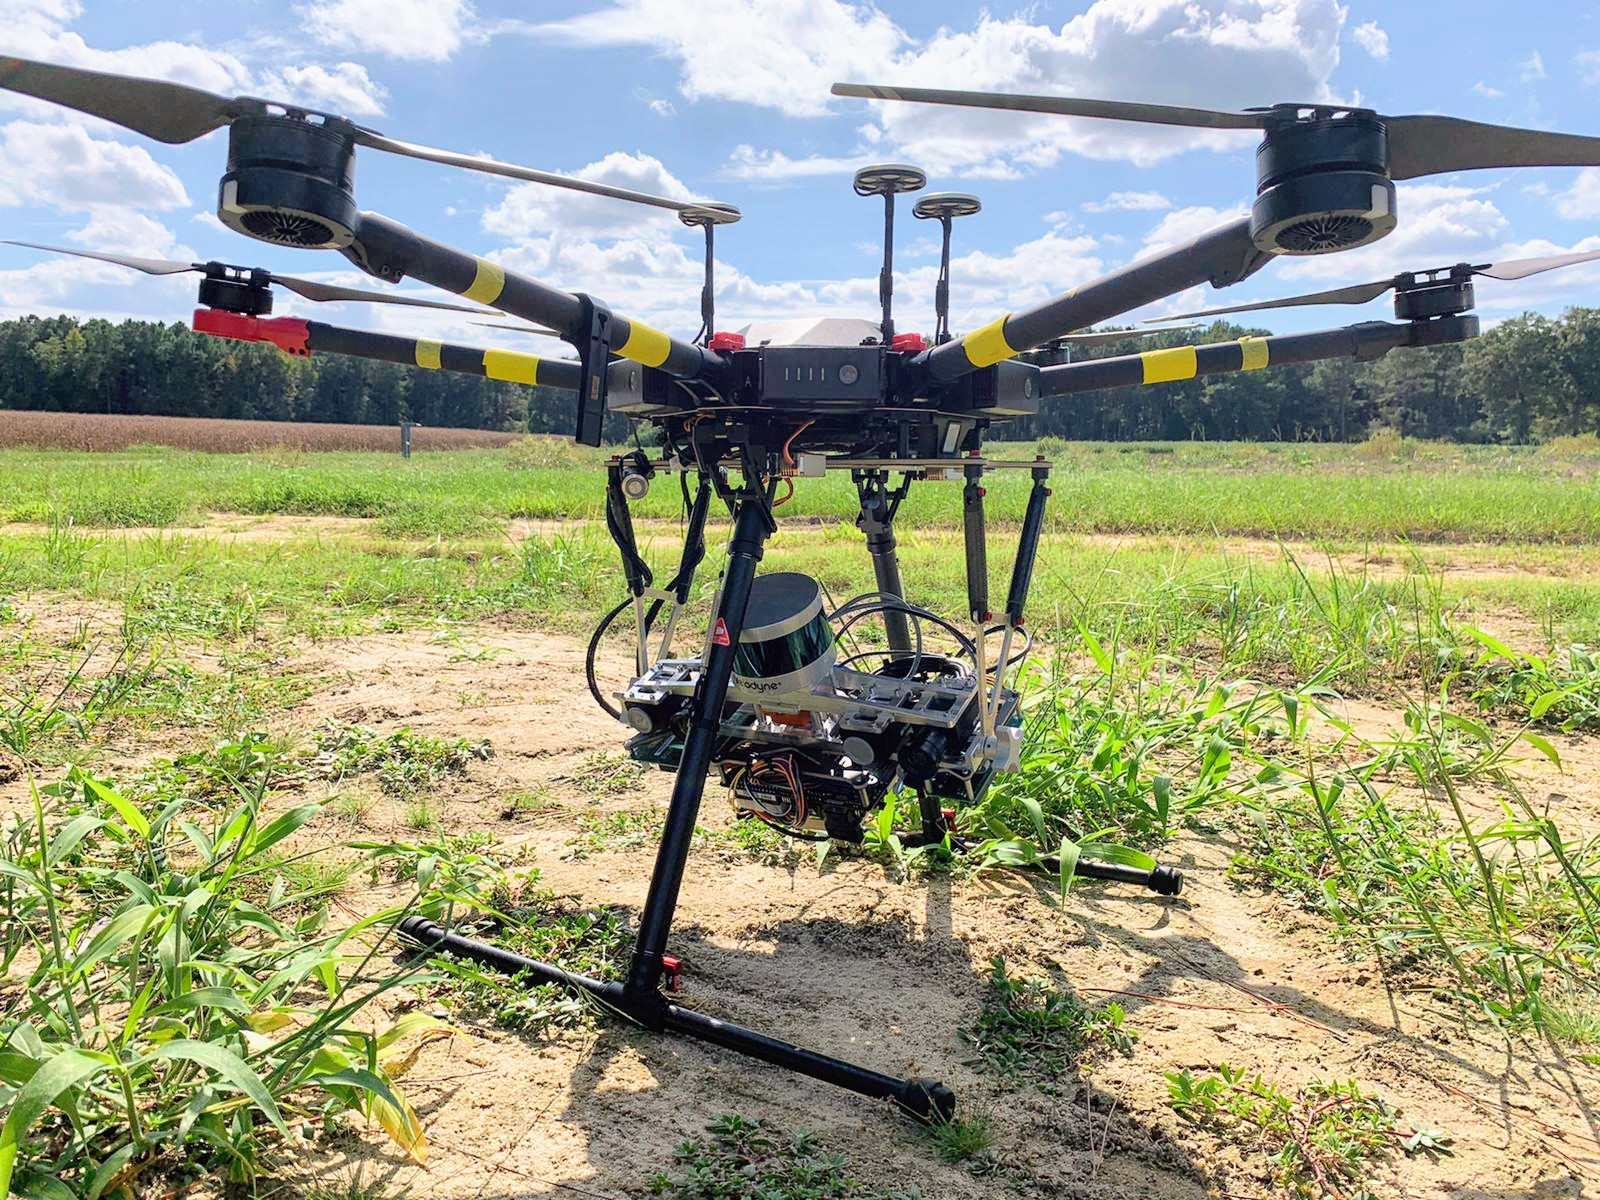
\includegraphics[width=0.37\textwidth]{figs/methods/datasets/payload_on_drone.jpeg}
    \caption{The multi-sensor payload designed by our collaborators. This was used for collecting rich forestry drone data. Photo credit to Winnie Kuang.}
    \label{fig:methods:payload}
\end{figure}

This payload is modular and could be mounted to different drones with different inclination angles. In these experiments, we used two large commercially-oriented drones, a DJI Matrice 600 and an AltaX Freefly. We flew a variety of different experiments, both under the canopy and over the canopy. In the under-canopy settings, we flew in small clearings between trees under manual control. Babak B. Chehreh from the University of Coimbra served as our pilot. In these experiments, we tried to survey the boundary of the clearing exhaustively by using an oblique payload orientation of 30 degrees from horizontal.

In the over canopy setting, we used a commercial flight planner. This allowed us to do a coverage plan over a region, using a traditional "lawnmower" pattern. Our altitude and overlap varied by experiment, but in most cases it was approximately 40 meters.


\begin{table}[]
\centering
\begin{tabular}{|l|l|l|l|l|}
\hline
\textbf{Name} & \textbf{Location} & \textbf{Platform} & \textbf{Environment} & \textbf{\makecell{Flight Pattern\\(camera degrees \\from horizontal)}}\\
\hline
Coimbra & \makecell{Coimbra,\\ Portugal} & \makecell{Multi-sensor \\ payload} & \makecell{Forest path} & \makecell{Manual out \\and back (30)} \\ 
\hline
Oporto & \makecell{Oporto,\\ Portugal} & \makecell{Multi-sensor \\payload} & \makecell{Forest clearing\\ with grass} & \makecell{Manual observations\\ of the boundary (30)}\\
\hline
Gascola & \makecell{Pittsburgh,\\ PA USA} & \makecell{Multi-sensor \\ payload}  & \makecell{Trees, shrubs,\\ and grasses} & \makecell{Lawnmower \\ over canopy\\ (75)} \\
\hline
Wharton & \makecell{Hammonton,\\ NJ USA} & \makecell{Multi-sensor \\ payload}  & \makecell{Forest with road} & \makecell{Manual oval \\ over canopy\\ (60)} \\
\hline
Stowe & \makecell{Stowe,\\ VT USA} & \makecell{DJI Air 2s} & \makecell{Forest} & \makecell{Lawnmower (90)} \\ 
\hline
%Emerald \cite{Young2022} & \makecell{Lake Tahoe,\\ CA USA} & \makecell{DJI Mavic 2} & \makecell{Forest} & \makecell{Lawnmower (90)} \\ 
%\hline
\end{tabular}
\caption{A summary of drone datasets used in this work.}
\end{table}

\subsection{Non-drone Forestry Data}
We also used two existing sources of forestry data that were relavent to our domain. The first was a dataset of 121 images of a Portugese forest taken from a ground vehicle in the work of Andrada et. al. \cite{Andrada2020}. These images were manually labeled with six classes: Background, Live flammable material (aka Fuel), Canopies, Trunks, Humans, and Animal The original paper uses multi-spectral data but we just used the co-registred RGB data that was also releasted. This choice allowed us to deploy the model on a normal camera, rather than requiring a multi-spectral one. We refer to this dataset as \textit{Sete Fontes} because it was collected in a region with that name.

We also used a synthetic dataset rendered from a proceedurally-generated Portuguese forest \cite{nunes2021procedural}. In this work, the authors proceedurally-created a forested landscape by first creating the terain, the placing paths and rocks, and finally adding vegitation. Then they rendred images from this mesh. At the same time, they also a semantic image, that perfectly captured which class was observed at each pixel. These classes were slightly more-granular than those used in \cite{Andrada2020}, but they could easily be aggregated to match these. The exception was there were no examples of humnas or animals in this simulated dataset, but these were also rare in the Sete Fontes dataset and were not critical to this work. The synthetic dataset consisted of 3154 rendered images and associated sematic segmentation groundtruths taken at intervals from a simulated ground vehicle trajectory. 

\subsection{Optical remote sensing data}
In this work, we focus primarily on data collected by the National Aerial Imagery Program (NAIP) multi-spectral data source which contains red, blue, green and near-infrared bands. This data is collected at an interval of at most every three years over the continental US. The USDA contracts with states to obtain this data from manned aerial surveys. The data is post-processed to provide an ortho-rectified, stitched, and georefernced product analogous to satellite imagery. The resolution per pixel is 0.6 meters, which is relatively high for a free data product with a significant extent. An example image can be seen in Figure \ref{fig:methods:NAIP_example}.

\begin{figure}
    \centering
    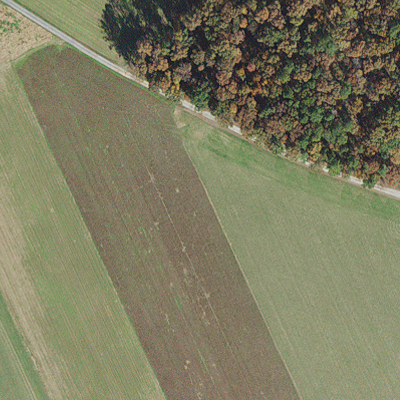
\includegraphics[width=0.5\textwidth]{figs/methods/datasets/NAIP_example.png}
    \caption{An example NAIP image crop.}
    \label{fig:methods:NAIP_example}
\end{figure}

\begin{table}[]
\centering
\begin{tabular}{|l|l|l|l|l|}
\hline
\textbf{Name} & \textbf{Location} & \textbf{Type} & \textbf{Environment} \\
\hline
Sete Fonte & \makecell{Coimbra,\\ Portugal} & \makecell{Under-canopy \\ images} & \makecell{Forest} \\ 
\hline
Synthetic \cite{nunes2021procedural} & \makecell{N/A, simulated} & \makecell{Under-canopy \\ images} & \makecell{Forest} \\ 
\hline
NAIP & \makecell{Continental US} & \makecell{Aerial imagery} & \makecell{Varied} \\ 
\hline
 Chesapeake LULC \cite{Claggett2014ChesapeakeProduction, Robinson2019LargeData} & \makecell{Chesapeake Bay,\\ US} & \makecell{Annotated \\ Land Use/\\Land Cover\\ classification} & \makecell{Varied} \\ 
\hline
\end{tabular}
\caption{A summary of non-drone datasets used in this work}
\end{table}

%\subsection{Data management}
%A practical consideration when dealing with this much data is how to effectively store, version, organize, and share it in a seamless fashion, especially when working in collaborative teams. The tool used for managing the complexities of software development, such as `git`, have similar goals but do not support managing large, non-text files. 
%Cloud hosting and local harddrives inenvitably become challenging to organize and do not natively support a versioning system, which makes them susceptible to accidental errors or duplicated data. 
%In this work, we leveraged a software tool called Data Version Control (DVC), which is designed for organizing data in large projects such as machine learning and data science. DVC acts as a management layer between a git-tracked project and an arbitrary remote storage device. Effectively, DVC creates light plaintext files which describe the real data. These a small files can be tracked by `git` and represent a full history of the project.  
%
%We created a `git` repo and associated `DVC` datastore for each project we worked on that had a different goal. Our organizational strategy evolved over time, but at the end involved two main concepts: a standardized hierarchy to organize the different data collects and a level designation to sort data based on the level of processing. The organizational structure was as follows `site\_name -> YYYY\_MM\_DD -> collect\_NNN` A site name represented one location where we collected data. This was chosen as the top-level organizational structure because data from the same site is most commonly used together. The next level represented the date and the final level broke the data up into logical segments. In general this corresponded to one drone flight, but in rare instances represented multiple flights where we left the sensors logging continuously, or data collected solely on the ground for calibration purposes. The level designation was inspired by the satellite community, where different levels denote different steps of sequential post-processing. In our work, we used Level0 to represent raw data, as copied from the platform. Level1 represented data processed into a standarized format. This was less important for commodity drone data, since it was frquently already captured as folders of geotagged images. However, it was very important for extracting easy-to-use information from rosbags, which is how our multi-sensor custom data was stored. Level2 represnted processed results such as structure from motion and semantic predictions. In initial work, we nested all the levels within a collect. However, we later found that for our usecases it was easier to have levels be the top level organizational structure. This allowed us to quickly check for all datasets matching a specific level of processing. The final organaiztional structure was as follows:
%
%% TODO fix this up
%
%\begin{verbatim}
%    
%├── level_00
%│   ├── README.md
%│   ├── <site_name_x> # A different folder for each geographic location
%│   │   └── <date_YYYY_MM_DD> # A different folder for each day at that site
%│   |       ├── collect_<NNN> # A different folder for each collect, which is probably synonmous with a flight
%│   │       └── collect_<NNN>
%│   └── <site_name_y>
%│       └── 2023_06_15
%│           ├── collect_<NNN>
%│           └── collect_<NNN>
%├── level_01 
%│   ├── README.md
%│   └── per_collect # Data in easy-to-use format, structured like level_00
%│       └── README.md
%└── level_02
%    ├── README.md
%    └── photogrametry # Photogramtery results
%        ├── README.md
%        └── metashape # Could have multiple softwares
%            └── per_collect # Structured like level_00
%\end{verbatim}

\section{Geometric understanding of forests using drone data}
\subsection{Photogrametry}
Data from commodity drones is very easy to use with structure from motion, since it is often provided as folder of images, with GPS information embedded in the EXIF metadata. This GPS information is not require, but provides a very helpful initialization to the structure from motion process. Furthermore, commodity drones are often set to only capture data at a low frequency or after traveling a given distance, to manage limited storage. Therefore, it is often advantageous to use all the available images. However, with our custom payload, the data was captured at a high frequncy of 10 HZ so consecutive images were often highly redundant. As shown by Young et. al. \cite{Young2022}, highly redundant images contribute little to the overall quality but we found them to dramatically increase computation times. Therefore, we the drone we downampled the image to 2HZ. If we had GPS data available, we tagged each image with the GPS coordinate from the temporally-nearest GPS record.   

After preliminary experiments, we found that a commercial software, Agisoft Metashape consistently produced high-quality results. We used the parameters found to work well by by Young et. al. \cite{Young2022}. In this study, the authors do not provide recommended parameters for the meshing step because this representation is not used in their pipeleine. Therefore, we used the default Metashape settings, which include "high" quality and "high" number of faces. In settings where we needed ortho-mosaics, or top-down renders, we also used the default settings. We conducted our experiments on high-end cloud infrastructure from the NSF Jetstream \cite{} program. 



\subsection{SLAM}    
Since SLAM is not the focus of this work, we choose to use results from our collaborators on these datasets. We use two methods from their experiments, LIO-SAM \cite{Shan2020LIO-SAM:Mapping} with the parameters tuned for the forestry domain and a custom SLAM that combines components of both LIO-SAM and VIL-SLAM \cite{Shao2019StereoMapping} to make an approach that combines information from both LiDAR and stereo vision in a tightly-coupled manner. A through description of this system can be found in \cite{RussellUnmannedMitigation}.

\section{Tree Detection in Top-Down Data}
The goal of this work is to study tree detection at multiple scales. We assume that we have data from three sources, low resolution aerial or satellite data, high resolution drone imagery, and the ground truth location and shape for the trees in a small region. The ground truth trees are assumed to be fully within the region the drone surveyed and the drone survey is assumed be be fully within the region with satellite data. This is a realistic model for a situation where a forester measured the trees in a region and then flew a drone to survey the surrounding area. The remote sensing data could be taken from any relevant available source, such as NAIP. An example of the scale of the different types of data can be seen in Figure~\ref{fig:methods:multi_scale_tree_det}. The goal of this study is to provide recommendations on how to use data at these three scales to detect trees as accurately as possible and determine whether all three are required. 

\begin{figure}
    \centering
    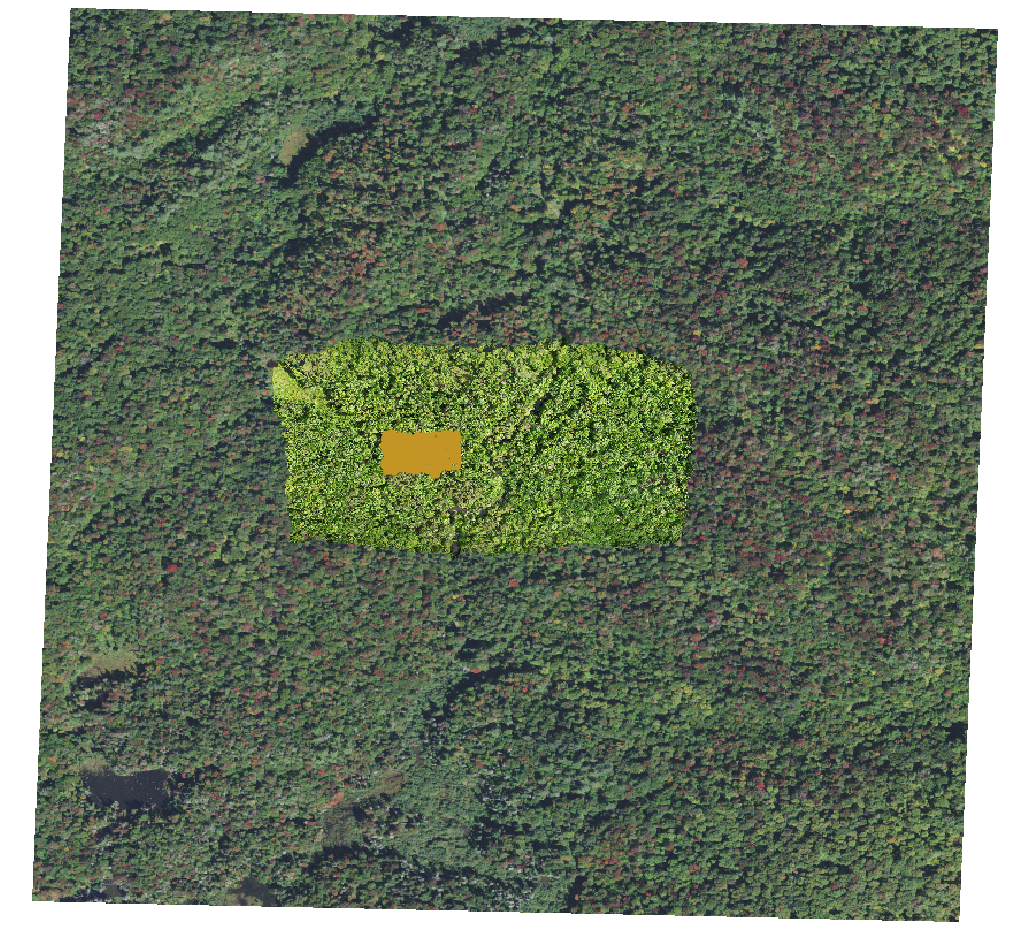
\includegraphics[width=0.3\textwidth]{figs/methods/tree_detection/multiscale_outset.png}
    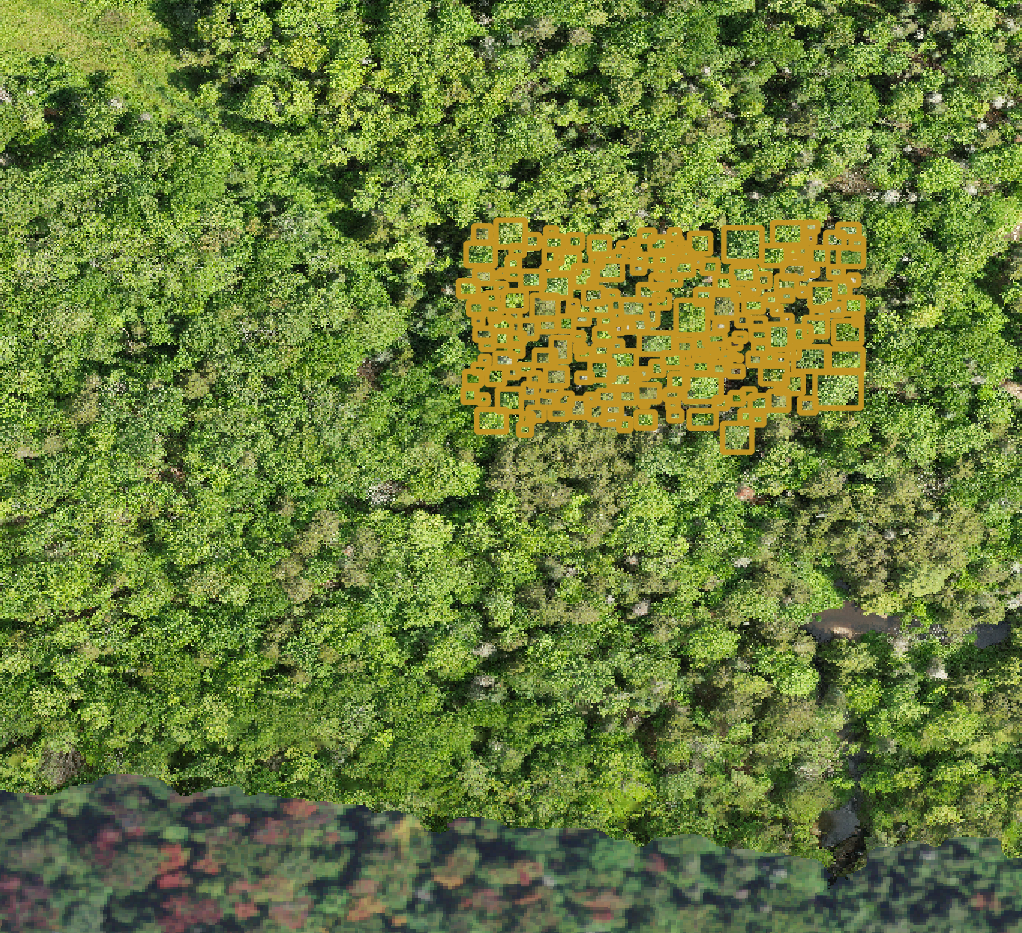
\includegraphics[width=0.3\textwidth]{figs/methods/tree_detection/multiscale_inset.png}
    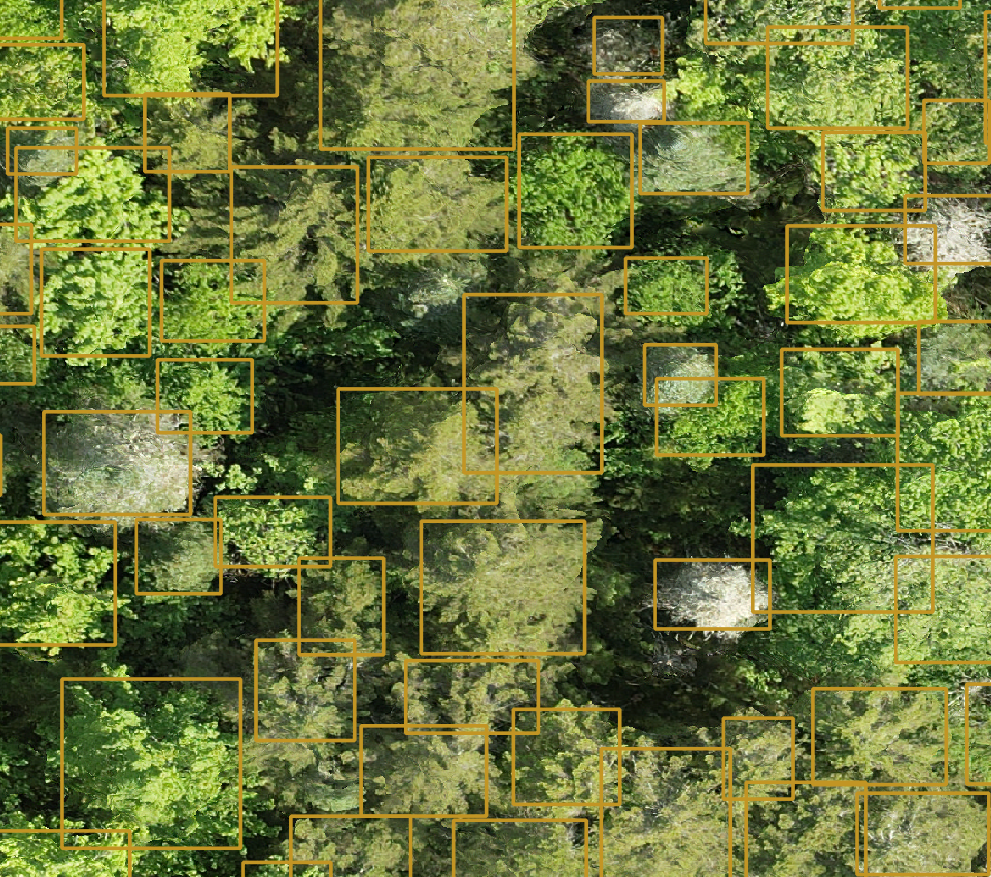
\includegraphics[width=0.3\textwidth]{figs/methods/tree_detection/multiscale_in_inset.png}
    \caption{The experimental setup with broad-coveraged aerial data, medimum coverage drone data and a small set of ground truth tree locations. The same data is visualized at three different scales for clarity.}
    \label{fig:methods:multi_scale_tree_det}
\end{figure}

The first step in this experiment was processing the drone images into an orthomosaic, as described in the Photogrametry section. This had a resolution of approximately 3 centimeters per pixel. Since the drone has GPS, this orthomosaic is roughly registered to a global reference frame. However, there is some noise and we noticed a slight mis-registration in both scale and translation. We precisely aligned the orthomosaic to our aerial data using QGis \cite{QGIS_software}. This provides an interface to select correspondences between the two datasets. Then, it optimizes a translation and scale transform to best align the two. 

In this work we used DeepForest \cite{Weinstein2020DeepForest:Delineation}, a widely-used deep tree detector based on deep learning.
The authors state that two parameters, spatial resolution and sliding window size, are especially important when applying DeepForest to new data. In preliminary experiments, we re-sampled the data to a variety of resolutions. We found that performance appeared best around the resolution that the model was trained on, 0.1 meters per pixel. Therefore we resampled both datasets to this resolution. This resulted in downsampling (coarsening) the drone data and upsampling (interpolating) the aerial data. We used the default window size of 400 pixels, which was also the size used for training.

The goal of our experiments is to answer two questions. The first is how valuable are the field reference measurements and drone collects. This would inform whether it is worth collecting these two additional types of data or if they can be safely omitted. The second is how to use all three data products together if they are available.

We propose a set of experiments to explore the these tradeoffs. The baseline approach is applying the pretrained DeepForest model to the aerial data. This requires no field measurements, but is expected to produce low-quality detections because the model was trained on drone data at native resolution, which has significantly more texture. The next approach is using the pretrained version of DeepForest on the drone data. This is expected to be significantly better than the aerial data because it is similar to what the model was trained on. The next two experiments involve fine-tuning the drone and aerial models on the small set of ground truth measurements. We expect that this fine-tuning will have a positive impact on the performance.

\section{Semantic Mapping of Forests}
The goal of our semantic mapping experiments was to determine what type of vegitation was where in the environment. We had a specific focus on accurately localizing fuel so that an automous ground robot could remove it. To accomplish this, we needed to both provide an accurate map of the world and add additional information to this map about what type of object was at each location.

Semantic mapping can be done with a variety of modalities. A relevant work on semantic mapping for forestry \cite{Chen2020SLOAM:Inventory}, focuses solely on detecting tree trunks within the environment. Because of the distinctive geometry of trunks, they are able to detect them in LiDAR. Because we want to distinguish classes that may have similar geometry, we choose to predict semantics using images, as done in the work of Andrada et. al. \cite{Andrada2020} in the ground vehicle setting. Using images has the added benefit that it is easy for humans to label annotated data to train the approach and to evaluate the quality of the predictions. Moreover, there is a wide range of semantic segmentation models available that are conceptually interchangeable. 

\subsection{Semantic Segmentation}
To the best of our knowledge, there are no pre-trained models that are useful for our task and publically available. Therefore, we needed to train our own models. We conducted two experiments, one on Portuguese data and another on the \textit{Gascola} we collected in the US. 

In the gascola experiemnts, our objective was to segment the different classes from overhead imagery. Since there weren't any relavent datasets, we chose to label a small ammount of data on our own for training. In semantic segmentation, it is very time consuming to label the boundaries between each class precisely. This is especially true for natural environments, where different classes are often interlaced at the boundary, such as tree branches over the ground or bare earth transitioning to grass. A relevant work on segmenting ground cover with drones is Davila et. al. \cite{Davila2022ADAPT:AI}, where they showed the coarsely labeling regions away from class boundaries was much faster and the model trained on these coarse annotaions still made good predictions at the boundaries. We conducted annotations using the VIAME toolkit, a free and open source web annotator pictured in Figure \ref{fig:methods:manual-annotations}. Even though our primary goal was to only distinguishes broad classes, we chose to annotate a more granular set of classes loosely inspired by the Anderson13 classes \cite{anderson1981aids}, a vegetation classification system commonly-used in fire modeling. Our reasoning was that this allowed us more flexibility when it came to future experiments, where we might want to aggregate the clsases differently. Furthemore, it gave us the option to train on these classes and aggreate them after prediction. In practice, we found that this additional granularity did not increase the labeling burden significantly, since we rarely had to break up spatial regions that would have originally been considered one coarse class. Rather, we mostly labeled entire regions with more granualar designations. 
To evaluate the performance of the model, we used another small annotated dataset from another flight over the same region. We summarized the IoU, precision, and recall for each class.

We use a segmentation network based on a transformer architecture called SegFormer \cite{Xie2021}. Given the relatively low amount of real-world images in our training dataset, this network was especially suitable since it showed strong performance on benchmark datasets and good generalization capabilities. We trained this model using the default parameters used in the MMSegmentation \cite{mmseg2020} implementation. 

Given the limited availability of real data and the labor-intensive nature of labeling to obtain ground truth, we explored the utility of models trained with simulated (\textit{synthetic}) data. We conducted three types of experiments: models trained solely with \textit{synthetic} data, models trained with real data (\textit{Setes Fontes}), and a mixture of both. For the last two cases, we trained with an increasing number of real images to evaluate the performance of the model with minimal real images. Thus, we conducted training experiments using (or adding) 7, 15, 21, 30, 60, 91, and 121 data points from the \textit{Setes Fontes} dataset. We trained for 10000 iterations and evaluated each model in 30 \textit{Setes Fontes} images not seen in the largest training split are used for evaluation and we replicate this experiment over five folds of the data. The three models are a fine-tuned implementation as the base networks were first trained with the \textit{CityScapes} dataset \cite{Cordts2016}.

\begin{figure}
    \centering
    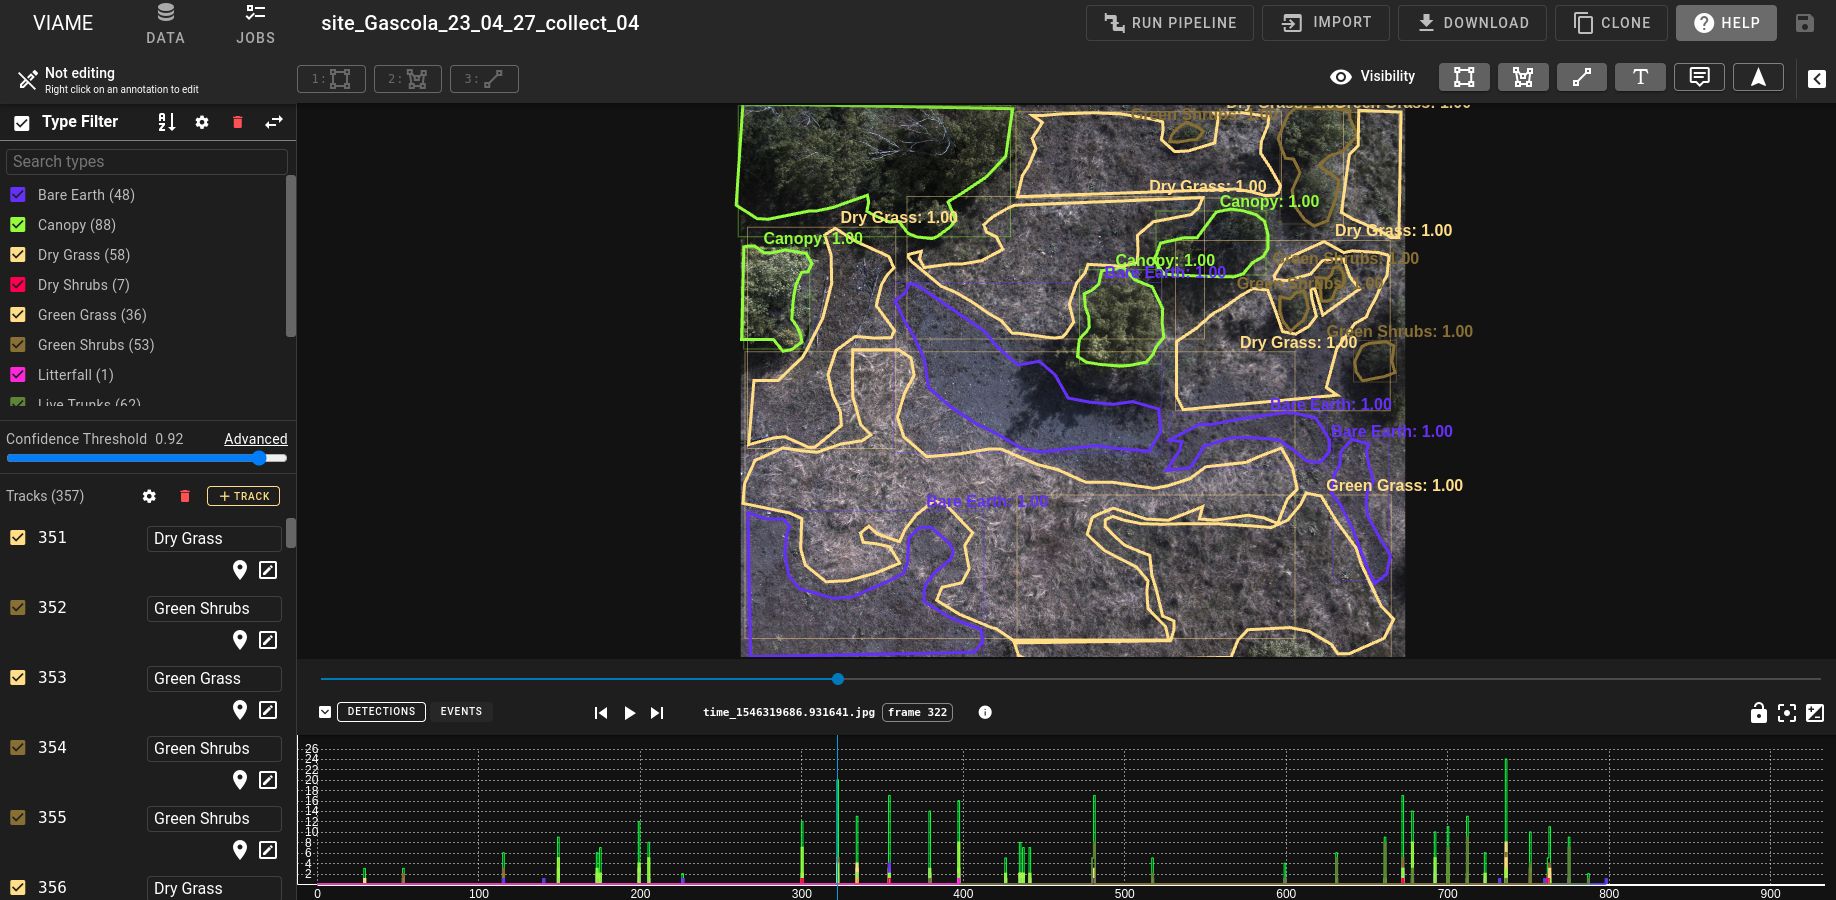
\includegraphics[width=\textwidth]{figs/methods/semantic_mapping/viame_example.png}
    \caption{Example manual annotations using the VIAME toolkit, a free and open source web annotator with potential support for integrated model training.}
    \label{fig:methods:manual-annotations}
\end{figure}

\subsection{Semantic Mapping with a Camera and LiDAR}

\begin{figure}
    \centering
    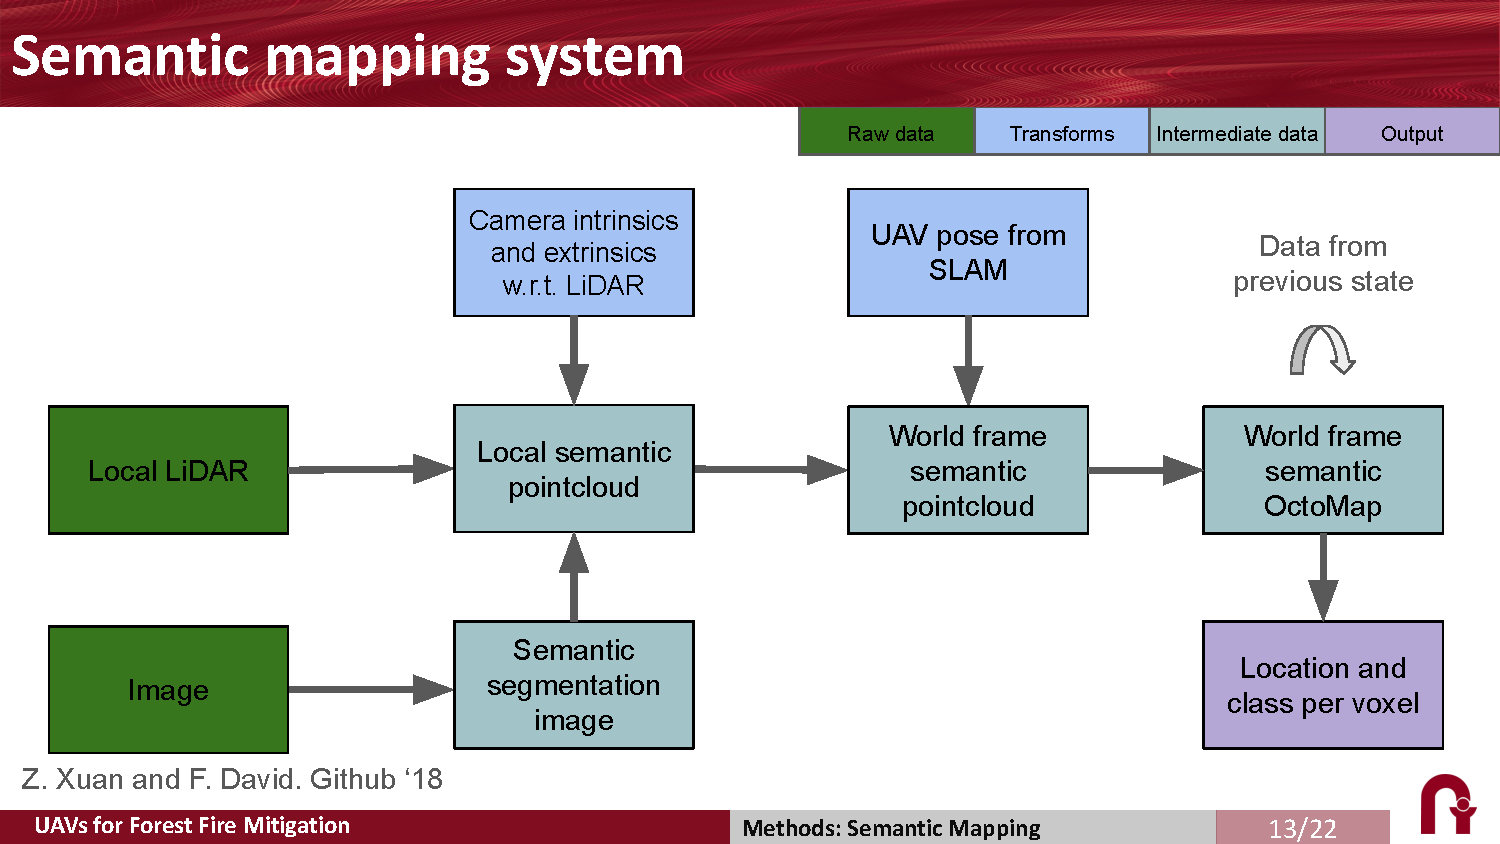
\includegraphics[width=\textwidth, clip, trim={0 1.5cm 0 1.8cm}]{figs/methods/semantic_mapping/semantic_mapping_overview.pdf}
    \caption{An overview of the LiDAR-camera semantic mapping system}
    \label{fig:methods:lidar-camera-semantic-mapping}
\end{figure}

We modified an approach for RGB-D semantic mapping \cite{semantic_slam} to project the segmentations from the image to the LiDAR domain (i.e., three-dimensional). First, the image is passed through the semantic segmentation network to get a classification result for each pixel. Using the extrinsics of the LiDAR relative to the camera, we transformed the LiDAR measurements into the camera's coordinate frame. Then, using the calibrated camera intrinsic, we project each LiDAR point into the image plane. Points within the field of view of the camera are assigned a classification label from the corresponding pixel in the semantic map. This semantically-textured point cloud is transformed into the inertial reference frame using the current pose of the drone estimated by our SLAM system. 

We use an octomap \cite{hornung13auro} representation to efficiently discretize the generated semantic point cloud into voxels. Each voxel has a resolution of 0.05m and contains information about the predicted classification. Each time a new semantic point cloud is created, it is used to update this global octomap. Since each voxel can contain multiple observations, we use two approaches to determine the aggregate classification. The first method assigns the class label using the highest-confidence prediction from the neural network that corresponds to that voxel. Alternatively, we use a Bayesian method which maintains a probability distribution over the classes. Each new observation is multiplied by the current distribution and then re-normalized. The voxel is then labeled with the most probable class. An overview of the proposed system can be seen in Figure \ref{fig:methods:lidar-camera-semantic-mapping}.

%\subsection{Adding semantics to meshes}
%\begin{itemize}
%    \item The semantics are predicted for each image
%    \item The semantics are predicted onto the mesh faces
%    \item They are aggregated across the different viewpoints using...
%
%\begin{figure}
%    \centering
%    \includegraphics{example-image-a}
%    \caption{Single-view semantic prediction}
%    \label{fig:single-view-semantic-pred}
%\end{figure}
%
%\end{itemize}





\section{Informative Path Planning}
% Motivate informative path planning and explain a little bit about the goals
A natural question is where to collect observations survey so that effectively extrapolate with satellite imagery to a broader region. 
Intuitively, the samples should be diverse and focus on examples which are expected to be the most interesting class or most challenging to classify. This intuition is challenging to implement in a domain-flexible way while also respecting operational considerations.
A major constraint is that drones have a finite battery life which governs the distance they can cover before returning home to have their battery replaced. This means that the distance of any one flight is bounded. Commodity drones do not expose the ability to allegorically control the drone in real time based on the sensor inputs, so the entire trajectory must be planned before the drone takes off.
We make some simplifying assumptions to define the type of observations we take. Specifically, we assume that the atomic observation is a plot, or a small lawnmower survey of a fixed square size. We further assume that the user specifies a fixed number of plots to visit. Since it will take a fixed amount of time to execute the plot surveys, the maximum available time to traverse between plots is the maximum time of a full flight minus the time taken to complete the surveys. The algorithm's decision variables are where to place these plots and in what order to visit them, subject to the maximum time available to traverse between them.


A good choice of plots depends heavily on the task that is being conducted. However, it's possible that the data may be used for multiple-purposes or the method of conducting the task has not been defined when the data is collected. To make our system as general as possible, we assume that in the absense of any other information, collecting a diverse and representative set of samples is desriable. To implement this concept, we need some notion of similarity that is applicable to a variety of domains and input data. We also need a planner that uses this description of diversity to plan a set of observation plots that are diverse and representative.


\subsection{Feature Extraction on Remote Sensing Data}
\begin{figure}
    \centering
    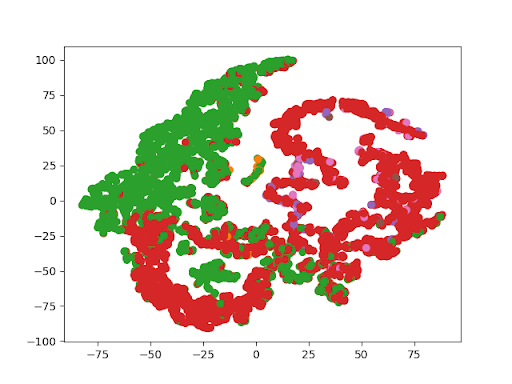
\includegraphics[width=0.5\textwidth]{figs/methods/IPP/TSNE_features.png}
    \caption{Unsupervised features seperate classes in a t-SNE embedding}
    \label{fig:methods:ipp_feature_embedding}
\end{figure}
Feature extraction is the process of converting raw data into a format that captures attributes that might be useful for machine learning. In classical computer vision, feature extraction or "feature engineering" was a widely-studied topic. Many works attribute the success of deep learning to the informative features that are extracted in early layers of the network. These are optimized for the target problem through the neural network training process. Since it takes a large amount of labeled data to train these features, it is common to use the first layers of a network trained for one task as a feature extractor or "backbone" for another related task that has less labeled data. However, applicable pre-trained models are not yet ubiquitous for remote sensing, especially given the diversity of modalities. Multiple approaches have been proposed to extract unsupervised features using paired modalities \cite{Xie2016TransferMapping} spatial correlations \cite{Jean2019Tile2Vec:Data} or layer-wise greedy training \cite{Romero2016UnsupervisedClassification}. In all cases, this still requires training a new network as a feature extractor which can be technologically difficult and computationally intensive.

A recent work called MOSAIKS \cite{Rolf2021} proposes random convolutional kernels as a strong alternative to pre-trained deep networks for feature extraction. Specifically, the suggest using small crops, e.g. 3x3, from the dataset as convolutional filters and then applying a non-linear activation. This process is extremely computational efficient and notably requires no neural network pretraining. Remarkably, the authors show that these features are remarkably good for a variety of predictions on geospatial data. Specifically, they are better than using a CNN as a feature extractor and almost as good as a CNN trained for the task in question.

Because of the strength and flexibility of this approach, we use it as the basis for our feature extraction method. The original work uses 1024 kernels to extract features, so it actaully increases the volume of data because the convolutional features are produced at the same resolution as the input image. In their work, they address this issue by spatially averaging the data across large cells. However, in our work, we require features that capture variation on a local level. Therefore, we retain the spatial resolution but reduce the number of features. This technique was employed in a related informative path planning work by Candela et. al., except the input was hyperspectral data rather than the convolutional feature maps. In both cases, the features are highly correlated with each other, so much of the information can be represented by a significanly-smaller number of features. We use Principal Component Analysis (PCA) \cite{Jollife2016PrincipalDevelopments}, a widely used statistical technique for reducing the dimensionality by finding the linear projection that retains the most variance in the original data. We use the first 6 principal components as features. A useful property of PCA is that the features it produces are uncorrelated. To make our feature representation even more consistent, we standardize each feature to have zero mean and unit variance. An example of feature extraction can be seen in Figure \ref{fig:methods:unsupervised_features}. This shows that different types of land cover have different feature representations.

\begin{figure}
    \centering
    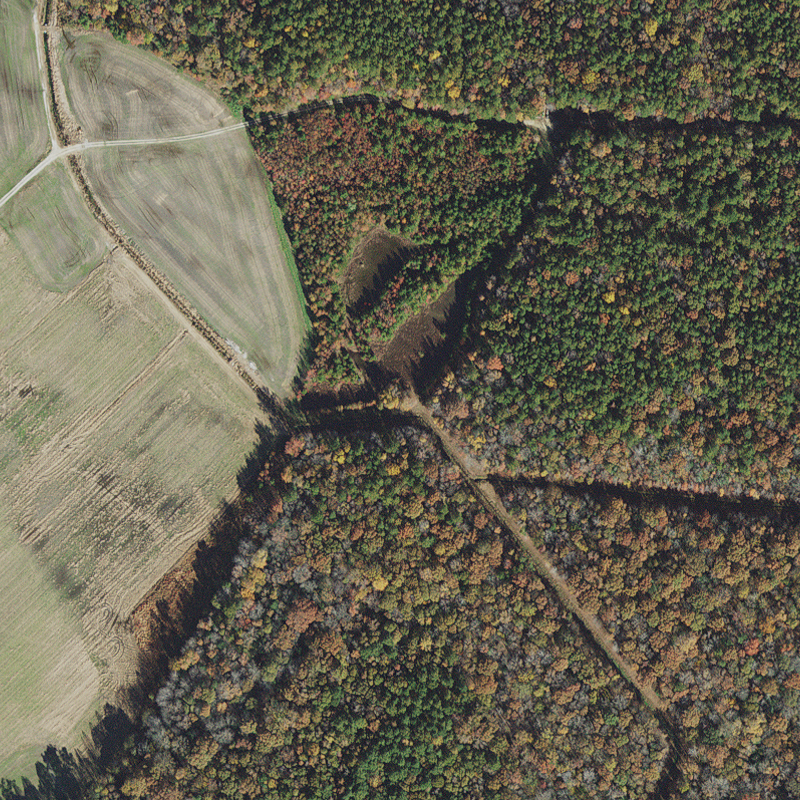
\includegraphics[width=0.3\textwidth]{figs/methods/IPP/img_for_features.png}
    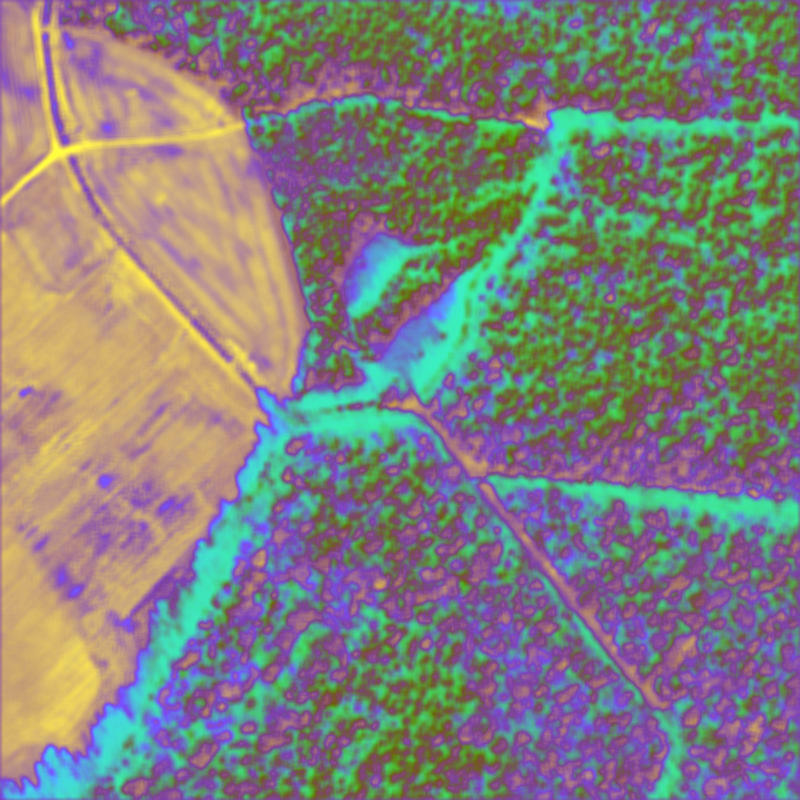
\includegraphics[width=0.3\textwidth]{figs/methods/IPP/first_three_feaures.png}
    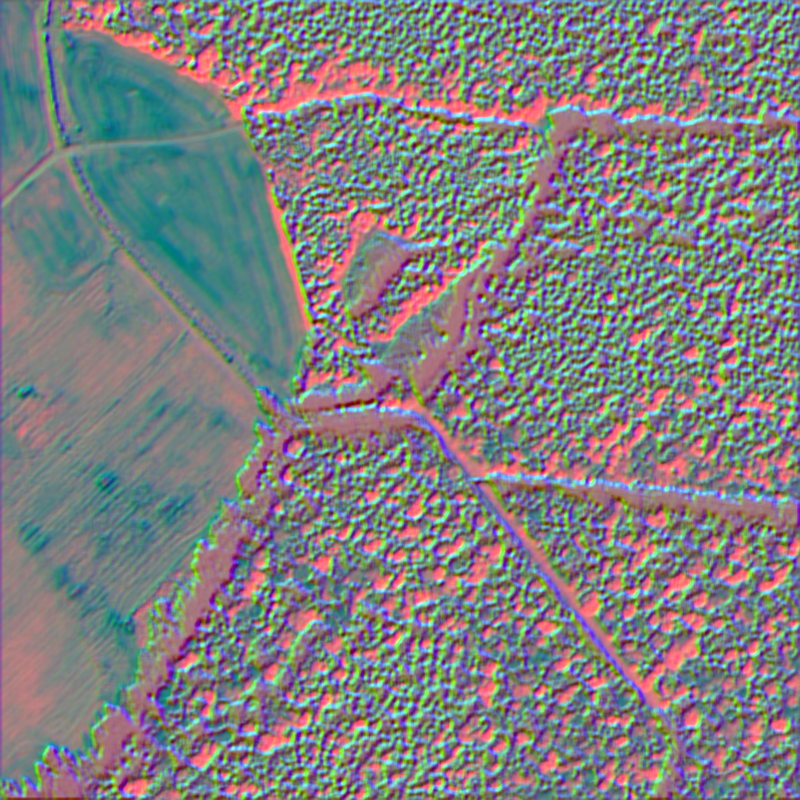
\includegraphics[width=0.3\textwidth]{figs/methods/IPP/second_three_features.png}
    \caption{Example unsupervised features generated by MOSAIKS and PCA. The first image is the input data and the next two images are the six features, visualized as the channels of two RGB images. For visualization, the data is centered at 0.5 and clipped at the third standard deviation.}
    \label{fig:methods:unsupervised_features}
\end{figure}


%As we continued to work on this project, and guided by the report feedback, we realized the value of a prediction system that is explicitly designed to work with very few training samples. This is specifically helpful if we want to collect a single set of labels and then train a preliminary model to inform the next round of sampling. While there are many approaches from the field of low-shot learning, they are often complex and tailored to a specific task and domain. To reduce the complexity of our approach and try to develop a generalizable method, we leverage Gaussian Processes (GPs) \cite{Rasmussen2004} implemented in \texttt{GPytorch}\footnote{\url{https://gpytorch.ai/}}. This prediction system is common in many related works because it provides an explicit uncertainty, which can be used to inform sampling, along with the prediction. While GPs are often used for regression tasks, extensions exist for classification, such as \cite{milios2018dirichletbased}, which is implemented in \texttt{GPytorch}.

%One major limitation of GPs is they are best suited to problems with several dozen features or fewer. Therefore, we must design a feature engineering strategy that produces useful features for these GPs to learn over. Directly using the channels of each satellite pixel does not capture the textures of the scene, which are important for moderately-high resolution data. While CNNs are commonly used for feature extraction, there is not the same diversity of pretrained models for satellite data as there are for other forms of imagery common in the computer vision community. However, recent work has shown than semi-random features are a strong alternative to even task-specific CNN features \cite{Rolf2021}. Specifically, this work proposes MOSAIKS, which are features computed by convolving random cropped patches of the image across the entire archive of satellite data. As shown in this work, these features are useful for a variety of downstream tasks. However, since the dimensionality of the feature vector is often in the hundreds or thousands (corresponding to the same number of randomly-sampled patches) it's too large to be used as an input to a GP. Therefore, we apply dimensionality reduction by using PCA to reduce the features down a reasonable number. In this case, we use 6. An example of this feature extraction method can be seen in Figure \ref{fig:unsupervised} and Figure \ref{fig:TSNE} shows that the features appear to separate nicely based on class.


    
\subsection{Gaussian Process Uncertainty Modeling}
Now that we have a strong feature representation, we begin to think about how to model uncertainty. Gaussian Processes (GPs) \cite{Rasmussen2004} are a principled tool for quantifying prediction uncertainty. They are a kernel-based method, where the kernel defines the similarity between two features. This can be fit to data or set using expert knowledge. Because of this, they are used as a key component of works on sensor placement \cite{Krause2008Near-optimalStudies} informative path planning \cite{Fernandez2022InformativeAnalysis, Candela2020PlanetaryMapping, Candela2021}. An important property of Gaussian Process uncertainty is that it only depends on the features and not the associated values. This makes them applicable to offline planning. 

 
\subsection{Long Horizon Informative Path Planning}
Now that we have addressed feature extraction and uncertainty modeling, we need an algorithm to plan a path that can effectively reduce the uncertainty. We make two observations that inform this work. First, drones can move in any direction and since we are flying above canopy, there are assumed to be no obstacles. Moreover, the drone has to stop down to execute each survey, so kinematic considerations are effectively removed. Given the scale of distances between points and drone's rapid acceleration, the time to traverse between points is assumed to be proportional to the distance between them.  

%We employ a sampling-based strategy to build a long-horizon map, with the goal of decreasing the uncertainty about the entire region. This work is related to RIG-Tree \cite{Hollinger2014Sampling-basedAlgorithms}, but is simpler, considers areas measurements at the vertices of traversals rather than edges, and directly optimizes for a path that returns to home under the alloted budget.


We employ a sampling-based strategy to build a long horizon offline path. This takes in an initial location, a number of samples, and a traversal budget. The algorithm begins by computing the Gaussian Process uncertainty after only observing the first location. Then, a feasible region is computed using a fraction of the remaining budget. A fixed number of samples are drawn from this feasible region, using a weighted sampling based on their uncertainty. The sample which reduces the total map uncertainty the most is added to the plan. Then the points are ordered using a TSP solver. The feasible region is recomputed using the added points and the fraction of the remaining budget.

\begin{figure}
    \centering
    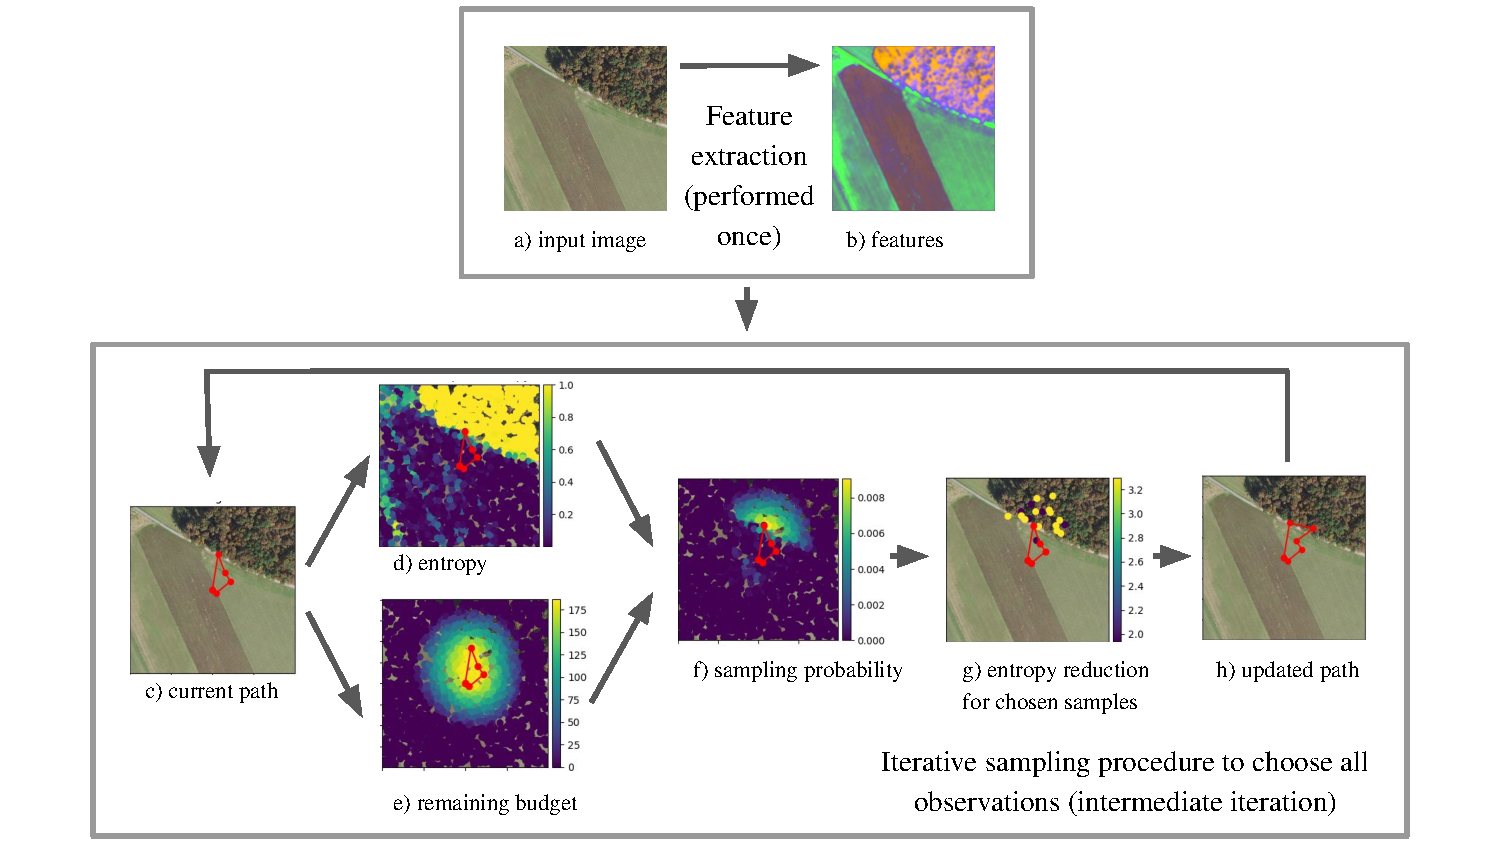
\includegraphics[width=\textwidth, clip, trim={1.5cm, 0, 1.5cm, 0}]{figs/methods/IPP/RAPTORS_concept_figure.pdf}
    \caption{This figure describes the workflow of a generalizable long-horizon path planner for selecting a set of drone observations. The required inputs are a satellite tile a), the drone's starting location, the path length budget, and the number of samples. Descriptive features are extracted from the image using random patches from the image as convolutional kernels, following the MOSAIKS method, and then compressed with PCA b). A full path is then built iteratively offline. At each iteration, the current path is provided as input, as shown in c). Then the uncertainty for a set of candidate locations is computed using a Gaussian Process d) and the remaining flight budget taking into account the current path is computed e). Then the uncertainty and remaining budget are multiplied and normalized to obtain a probability of evaluating each sample further. A set of samples are selected and the entropy reduction is calculated if each one were added to the Gaussian Process model f). Then the best sample is added and the path ordering is recomputed using a traveling salesman solver g). Then the process is repeated to plan the next observation until the requested number of observations are planned for. Only then is the path executed by the drone.
}
    \label{fig:methods:IPP_raptors_overview}
\end{figure}

%\begin{algorithm}
%\caption{RAPTORS}\label{alg:methods:RAPTORS}
%\begin{algorithmic}
%\State $F = extract\_features(I)$
%\end{algorithmic}
%\end{algorithm}
%
%\begin{algorithm}
%\caption{extract\_features}\label{alg:methods:extract_features}
%\begin{algorithmic}
%\State $F = extract\_features(I)$
%\end{algorithmic}
%\end{algorithm}
%
%\begin{algorithm}
%\caption{choose\_next\_sample}\label{alg:methods:choose_next_sample}
%\begin{algorithmic}
%\State $F = extract\_features(I)$
%\end{algorithmic}
%\end{algorithm}




\subsection{Experimental Setting}
The goal of this experiment is to simulate a land cover mapping mission for a region that is too large for the drone to exhaustively survey. Remote sensing data is available beforehand and is used to both inform the mission and generate predictions on the unobserved regions. In this experiment, we use NAIP data and manual land cover classification annotations from the Chesapeake Bay \cite{Claggett2014ChesapeakeProduction}.

%The goal of the experiments is to model a realistic data collection scenario. The data is collected over a series of missions, where each mission must be fully planned before it is executed. Each mission is allowed a pathlength budget and a number of samples it is allowed to collection. 

In our experiments we use randomly-sampled NAIP tiles to evaluate the approach. In each situation the agent starts in the center of the environment and must return there after each mission.

In these experiments we use a very simple prediction system to predict the class of unobserved pixels. It is simply a nearest-neighbor classifier which operates on the same PCA-compressed MOSAIKS features that are used for planning. While simple, this approach is well-suited to the extremely low number of training samples used in this setting and the standardized and uncorrelated nature of our feature space.

Before any missions have been executed, the agent can only observe the label of the pixel it is at. Then it plans a mission and executes it, observing the labels at the chosen sampling locations. These samples are used to train a prediction model which is used for evaluation and, in theory, could be used to inform the plan for the next mission. 


The experiments were conducted over ten random domains, which each represented an 800x800px crop from the Chesapeake Bay land cover dataset. Each tile represents approximately half a kilometer square. The pathlength was set as 800 pixels as well, which meant that the agent could go to one side of the environment and return to the start within the budget but some corners were completely unreachable. Each domain was explored using four missions where 10 samples could be collected during each one. Each sample meant the agent could observe the class of one pixel. After each mission, the class of all pixels  were predicted using the nearest neighbor classifier and the error metrics were computed. 


\subsection{Metrics}
The quality of the predictions are evaluated on two metrics, accuracy and averaged recall. The first is simply the fraction of pixels in the map that were assigned the correct class label by the prediction system. The second represents the average of the per class recalls. This metric is chosen so that rare classes are treated equally in the evaluation procedure, since this is critically important when we explicitly want to find rare classes. We also report the time taken to generate the plan. Note that this does not include the time taken to generate the class predictions, since the planner is agnostic to the choice of prediction algorithm.

 
% \begin{itemize}
%     \item Talk about this in far more detail
%     \item Add some more figures to describe the process
%     \item Finish algorithm descriptions
% \end{itemize}

\chapter{Experiments} \label{chapExperiments}


\chapter{Results} \label{chapResults}
\section{Quantitative evaluation}
\begin{itemize}
    \item Demonstrate that this planner does better than comparable batch planners in a head-to-head comparison
    \item Demonstrate that this planner does almost as well as online planners 
    \item Show the sensitivity to different algorithm configurations 
    \item Show the timing results, across different configurations
\end{itemize}

\section{Quantitative results}
\begin{itemize}
    \item The domain expert said this about our system 
    \item Here's the pretty result you get from our system
\end{itemize}

\begin{figure}
    \centering
    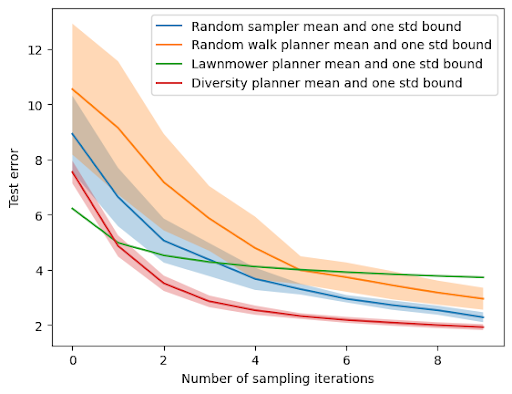
\includegraphics[width=\textwidth]{figs/results/GP_performance.png}
    \caption{This planner does better than everything else}
    \label{fig:quantitative}
\end{figure}

\begin{figure}
    \centering
    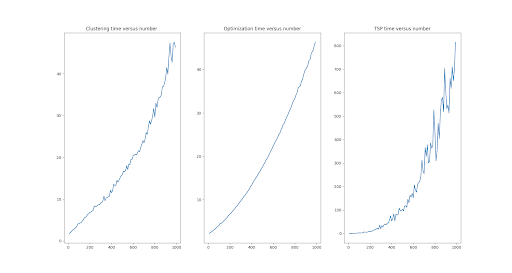
\includegraphics[width=\textwidth]{figs/results/timing.png}
    \caption{This is how long it takes to run each part}
    \label{fig:timing}
\end{figure}

\begin{figure}
    \centering
    \includegraphics[width=\textwidth]{example-image-a}
    \caption{Sensitivity analysis}
    \label{fig:sensetivity}
\end{figure}

\begin{figure}
    \centering
    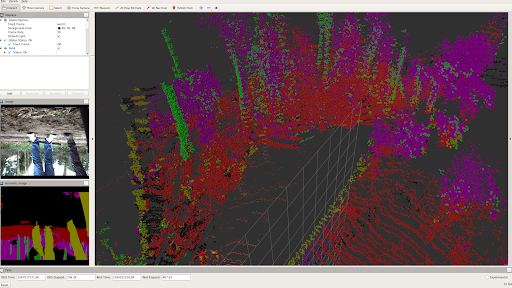
\includegraphics[width=\textwidth]{figs/results/semantic_mapping.png}
    \caption{You get this pretty thing when you run our system}
    \label{fig:pretty_thing}
\end{figure}

% -*- mode:LaTex; mode:visual-line; mode:flyspell; fill-column:75-*-

\chapter{Conclusions} \label{chapConclusions}
\section{Key Takeaways}S
We find that the structure from motion parameters suggested by Young et. al. \cite{Young2022} work well for reconstructing a number of diverse datasets. The performance is the best when the drone conducts a lawnmower survey above the canopy but manual non-overlapping flight can produce acceptable results. It is more challenging to generate reconstructions from images taken under-canopy, but further research may be able to address this issue.

We compare the performance of tree detection from both drone and remote-sensing data. The detections from drone data are still significantly better than those from NAIP data, even after resampling to the same resolution. 

This work demonstrates an approach to map the location of different types of vegetation using a drone equipped with a camera and LiDAR. We show that recent transformer-based semantic segmentation models are able to achieve moderate performance when trained on very few images from a target region.

We show that unsupervised feature extraction is a powerful tool for land-cover classification from remote sensing data. Specifically, using the approach described in MOSAIKS and compressing these features with PCA yields a compact and informative representation. These features can be used to plan informative drone flights by samples that minimize Gaussian Process uncertainty about the whole region.  


%\begin{itemize}
%    \item Structure from motion is a powerful tool to build 3D maps from drone images with minimal assumptions
%    \item A small amount of annotated data can be very useful to train deep learning models for a given natural environment
%    \item Predicting trees at increasingly-low resolutions yields better results 
%\end{itemize}
\section{Contributions}
This work makes two main contributions
\begin{itemize}
    \item We present a system for mapping different types of vegetation using multi-senors  SLAM for geometric information and vision-based semantic segmentation to differentiate vegetation classes. This has applications to forest fire mitigation and we believe this is the first system of its kind to address this problem. 
    \item We propose a novel long-horizon informative path planner that is applicable for planning surveys with commodity drones. We demonstrate that this method is an effective approach for choosing samples for a land-cover classification task.
\end{itemize}

%\begin{itemize}
%    \item Adding semantics to meshes 
%    \item Adding height information to semantics and tree detection images
%    \item Automatically registering data at different scales using trees as features
%    \item Evaluating the performance of different feature extractors
%\end{itemize}
        
\section{Proposed Concluding Experiments}
There are several additional experiments that we anticipate completing before the conclusion of this thesis.
For tree detection, it is clear that we need a quantitative assessment to better understand the tradeoffs between these different approaches.We plan to conduct a two-fold evaluation scheme by repeating the same steps we did on \textit{Stowe} on another dataset we collected in the same region. Then, we will evaluate the predictions from approaches trained on one location on the other, and vice versa, to get an accurate assessment of the ability of these approaches to generalize. We also propose to add two more experiments to the existing ones. These involve fine-tuning a model for aerial data on predicted tree locations from the drone data. In one case we used predictions from the pretrained model and in the other case we use predictions from the fine-tuned model. We hypothesize that this multi-stage approach will increase performance because of the increased diversity of training examples.  

We also would like to more thoroughly evaluate the sensitivity of RAPTORS to different parameter choices. We will first begin by assessing the impact of different parameters on the feature extraction side and different machine learning models for land cover predictions. Once we have settled on a desirable combination, we will run system-level experiments on the RAPTORS algorithm. Since these experiments are relatively computationally intensive, we will explore a number of parameters at once using randomized sampling. We will also test the algorithm on data from more diverse geographic regions.

\section{Future work}
In this work, we have demonstrated an online semantic mapping system that uses a custom multi-sensor payload. We are interested in extending this approach to commodity drones by using only GPS-tagged images as input to further increase the accessibility of this approach. Fortunately, this work and others demonstrates the ability of structure from motion to predict the geometry of forests from images alone. Therefore, semantic meshes \cite{} appear to be a promising approach, since they aggregate single-view semantic segmentation predictions onto the geometry of a mesh. As an additional improvement, geometric data from the meshes could be used to augment the visual data for semantic segmentation. For example, the height of the mesh corresponding to each pixel on the image could be computed using rendering techniques. Then this data could be concatenated with the visual imagery to provide a richer representation. This could help address ambiguities that are challenging to address from visual cues alone, such as the similarity between canopy and fuel at ground level.  





%\appendix
%\input{thesis-appendix}

% ********************************************************************************
%                                 Back Matter
% ********************************************************************************

\backmatter

% Normal line spacing
\singlespace

% By default \bibsection is \chapter*, but we really want this to show
% up in the table of contents and pdf bookmarks.
\renewcommand{\bibsection}{\chapter{\bibname}}
% Additionally, redefine the chapter header to remove the chapter number.
\renewcommand{\chaptermark}[1]{%
  \markboth{\color{headergray}{#1}}{}
}


%\newcommand{\bibpreamble}{This text goes between the ``Bibliography''
%  header and the actual list of references}
\bibliographystyle{plainnat}

% No whitespace allowed in the reference files list, ever.
\bibliography{bibliography/mendeley,bibliography/references}
\end{document}
